\chapter{动力系统与状态估计}
\label{chap:dynamical-systems-and-state-estimation}

第~\ref{chap:matrix-analysis}章已经说明，矩阵会沿不同方向放大或压缩向量； 第~\ref{chap:probability-theory}章建立了条件分布与条件高斯计算；
第~\ref{chap:stochastic-processes-and-approximation}章则把相关观测和随机更新放进时间序列。
这些工具还没有回答一个共同问题： 当一个系统把过去压缩进当前状态，并继续随时间演化时，
初值、输入、噪声和观测分别决定了什么？

第~\ref{chap:signal-analysis}章从输入到输出的整体关系出发，把线性时不变递推展开成卷积核。
该章以$\bm{s}_{t}$、$\bm{x}_{t}$、$\bm{y}_{t}$分别表示状态、输入和输出； 本章为突出状态估计，
把它们依次改记为$\bm{x}_{k}$、$\bm{u}_{k}$、$\bm{y}_{k}$，并先采用没有直接输入输出通道的观测方程。
本章转而保留递推中的内部状态。 状态不是对历史的逐项存档，而是足以继续预测未来的当前摘要。
给定初值和输入，状态方程决定一条轨迹； 加入过程噪声后，它决定轨迹的分布； 只能看到带噪观测时，还要用观测历史形成状态的条件分布。
这三个对象不能混用。

贯穿前五节的离散线性状态模型为
\begin{align}
	\bm{x}_{k+1} & = \bm{A}_{k}\bm{x}_{k}+\bm{B}_{k}\bm{u}_{k}+\bm{w}_{k}, \label{eq:dynamical-linear-state-model} \\
	\bm{y}_{k}   & = \bm{C}_{k}\bm{x}_{k}+\bm{v}_{k}. \label{eq:dynamical-linear-observation-model}
\end{align}
其中$\bm{x}_{k}\in\mathbb{R}^{d}$是状态， $\bm{u}_{k}\in\mathbb{R}^{m}$是给定输入，
$\bm{y}_{k}\in\mathbb{R}^{p}$是观测。
本章先令噪声为零，研究方程怎样产生轨迹、怎样数值计算，以及扰动会不会衰减；
随后恢复噪声，推导有限时域的预测、Kalman滤波与RTS平滑。

后半章改变问题对象：随机参数更新的长期趋势形成平均动力学， 离散随机增量进一步推进到连续时间，Hamilton动力学则研究怎样保持能量与体积。
轨迹稳定、状态估计准确、随机更新收敛和采样分布正确分别需要不同条件； 本章将把这些条件放在相应结论附近。

\section{由状态与输入确定轨迹}
\label{sec:dynamical-difference-ode}

\subsection{状态、初值与泄漏记忆}

先看一个带泄漏的标量记忆。 给定输入序列$(u_{k})$，令
\begin{equation}
	x_{k+1}=a x_{k}+b u_{k}, \qquad x_{0}\ \text{给定}. \label{eq:dynamical-leaky-discrete-memory}
\end{equation}
反复代入可得
\begin{equation}
	x_{k}= a^{k}x_{0}+ \sum_{j=0}^{k-1}a^{k-1-j}b u_{j}. \label{eq:dynamical-discrete-variation-constants}
\end{equation}
当前状态把初值和全部旧输入压缩成一个数。 当$|a|<1$时，较早输入的权重按几何速度衰减；
当$|a|>1$时，同一递推会放大早期扰动。 因此，“能够写成卷积”只说明计算结构，
并不保证记忆稳定。

例如令$a=1/2$、$b=1$、$x_0=0$，只在第零步输入$u_0=1$，后续输入都为零。
状态依次为$x_1=1,x_2=1/2,x_3=1/4$：一个脉冲留下的影响逐步衰减。
若第一步和第二步都输入$1$，则$x_2=3/2$，其中$1/2$来自旧输入，$1$来自新输入。
状态的“记忆”就是这些历史贡献的当前总和，不是把全部历史样本逐项保存下来。


若观察间隔缩短到$\Delta t$，可把泄漏系数写成 $a=1-\lambda\Delta t$，输入系数写成$b
=\Delta t$。 两边减去$x_{k}$并除以$\Delta t$，形式上得到
\[
	\frac{x_{k+1}-x_{k}}{\Delta t}= -\lambda x_{k}+u_{k}.
\]
当输入来自连续函数$u(t)$且极限存在时， 对应的连续时间模型是
\begin{equation}
	\dot{x}(t)=-\lambda x(t)+u(t). \label{eq:dynamical-leaky-continuous-memory}
\end{equation}
差分方程直接规定相邻时刻的更新， 常微分方程（ordinary differential equation, ODE）则规定每个时刻的瞬时变化率。
从后者得到可计算递推还要选择离散化方法， 不能把式~\eqref{eq:dynamical-leaky-discrete-memory}与
式~\eqref{eq:dynamical-leaky-continuous-memory}视为天然相同。

\subsection{初值问题的存在、唯一性与延拓}

一般一阶ODE初值问题写成
\begin{equation}
	\dot{\bm{x}}(t) = \bm{f}(t,\bm{x}(t),\bm{u}(t)), \qquad
	\bm{x}(t_{0})=\bm{x}_{0}. \label{eq:dynamical-general-ivp}
\end{equation}
给定输入$\bm{u}$以后，可以把右侧看成$(t,\bm{x})$的函数。瞬时变化率可能只在
几乎处处存在；要保证它仍能恢复整条轨迹，需要比普通连续性更强的条件。
\begin{definition}[绝对连续曲线]
\label{def:dynamical-absolutely-continuous-curve}
在有限区间$[a,b]$上，曲线$\bm x:[a,b]\to\mathbb R^d$称为
\term{绝对连续曲线}（absolutely continuous curve），如果存在
$\bm v\in L^1([a,b];\mathbb R^d)$使对所有$t\in[a,b]$都有
\(\bm{x}(t)=\bm{x}(a)+\int_a^t\bm{v}(s)\,\mathrm{d}s\)。此时$\dot{\bm x}=\bm v$几乎处处成立。
\end{definition}
因此，ODE的解不是任意满足局部斜率的点集，而是一条绝对连续曲线，并在几乎处处取
\(\bm{v}(t)=\bm{f}(t,\bm{x}(t),\bm{u}(t))\)，等价地满足积分方程
\begin{equation}
	\bm{x}(t) = \bm{x}_{0}+ \int_{t_0}^{t}\bm{f}(s,\bm{x}(s),\bm{u}(s))\,\mathrm{d}
	s. \label{eq:dynamical-ivp-integral-form}
\end{equation}

\begin{theorem}[局部存在唯一性]
	\label{thm:dynamical-picard-lindelof} 若$\bm{f}(t,\bm{x},\bm{u}(t))$在 $(t_{0},
	\bm{x}_{0})$附近关于$t$连续， 并且关于$\bm{x}$局部Lipschitz，其Lipschitz常数可在该时间邻域内统一选取，
则存在包含$t_{0}$的时间区间，
	使初值问题~\eqref{eq:dynamical-general-ivp}在该区间上有唯一解。
\end{theorem}

\begin{proof}
	记$\bm{g}(t,\bm{x})=\bm{f}(t,\bm{x},\bm{u}(t))$。
	取$a,b>0$，使闭区域
	\[
		[t_0-a,t_0+a]\times
		\{\bm{x}:\lVert\bm{x}-\bm{x}_0\rVert_2\leq b\}
	\]
	包含在定理的适用邻域内。记$\bm{g}$在该区域上的上界为$M$，关于$\bm{x}$的
	Lipschitz常数为$L$。选择$h>0$使
	\[
		h\leq a,\qquad Mh\leq b,\qquad Lh<1,
	\]
	并令$I=[t_0-h,t_0+h]$。连续曲线集合
	\[
		\mathcal{X}
		=
		\left\{
			\bm{z}\in C(I,\mathbb R^d):
			\lVert\bm{z}-\bm{x}_0\rVert_\infty\leq b
		\right\}
	\]
	是完备空间$C(I,\mathbb{R}^d)$的闭子集，因而仍然完备。在$\mathcal{X}$上定义
	Picard算子
	\[
		(\mathcal{T}\bm{z})(t)
		=
		\bm{x}_{0}+\int_{t_0}^{t}\bm{g}(s,\bm{z}(s))\,\mathrm{d}s.
	\]
	对任意$\bm{z}\in\mathcal{X}$和$t\in I$，
	\[
		\lVert(\mathcal{T}\bm{z})(t)-\bm{x}_0\rVert_2
		\leq M|t-t_0|
		\leq Mh
		\leq b,
	\]
	所以$\mathcal{T}$把$\mathcal{X}$映回自身。对任意两条候选曲线，
	\[
		\lVert\mathcal{T}\bm{z}_{1}-\mathcal{T}\bm{z}_{2}\rVert_{\infty}
		\leq
		Lh\lVert\bm{z}_{1}-\bm{z}_{2}\rVert_{\infty}.
	\]
	这里$h$是区间相对于$t_0$的半宽，因而压缩因子是固定常数$Lh$。
	由$Lh<1$，$\mathcal{T}$是压缩映射。压缩映射定理给出唯一不动点，
	而不动点正是积分方程~\eqref{eq:dynamical-ivp-integral-form}的解。
\end{proof}

局部Lipschitz条件服务于唯一性。 只有连续性时，解可能存在却不唯一。 例如$\dot{x}=\sqrt{|x|}$、$x
(0)=0$既允许恒为零的解， 也允许先停留一段时间再离开零点的解。
局部解也不自动延伸到任意时间。 方程$\dot{x}=x^{2}$从$x(0)=1$出发的解为$x(t)=1/(1-
t)$， 它在$t=1$有限时间爆炸。

若$\bm{f}$关于$\bm{x}$全局Lipschitz， 并且$\lVert\bm{f}(t,\bm{0},\bm{u}(t))\rVert$在有限时间区间可积，
Gronwall不等式可排除有限时间爆炸，从而把解延伸到所需区间。 更一般地，也可以用径向无界的能量函数证明轨迹留在有界集合。
因此，全局解依赖增长控制，而不只是局部导数存在。

\subsection{线性状态转移与常数变易公式}

连续时间线性时不变系统写成
\begin{equation}
	\dot{\bm{x}}(t) = \bm{A}\bm{x}(t)+\bm{B}\bm{u}(t). \label{eq:dynamical-lti-continuous}
\end{equation}
第~\ref{sec:matrix-analysis-functions-structured-operations}节定义的矩阵指数满足
\[
	\frac{\mathrm{d}}{\mathrm{d}t}\mathrm{e}^{t\bm{A}}= \bm{A}\mathrm{e}^{t\bm{A}},
	\qquad \mathrm{e}^{0\bm{A}}=\bm{I}.
\]
令$\bm{z}(t)=\mathrm{e}^{-t\bm{A}}\bm{x}(t)$， 乘积求导给出
\[
	\dot{\bm{z}}(t) = \mathrm{e}^{-t\bm{A}}\bm{B}\bm{u}(t).
\]
积分后再乘回$\mathrm{e}^{t\bm{A}}$，得到
\begin{equation}
	\bm{x}(t) = \mathrm{e}^{(t-t_0)\bm{A}}\bm{x}_{0}+ \int_{t_0}^{t}\mathrm{e}^{(t-s)\bm{A}}
	\bm{B}\bm{u}(s)\,\mathrm{d}s. \label{eq:dynamical-lti-variation-constants}
\end{equation}
第一项传播初值，第二项累计各时刻输入经过剩余时间后的影响。
这正是连续状态方程产生卷积核的来源。
为核对这个公式，记右侧为$\widetilde{\bm{x}}(t)$。代入$t=t_0$可得
$\widetilde{\bm{x}}(t_0)=\bm{x}_0$；再用积分上限求导，
\[
	\dot{\widetilde{\bm{x}}}(t)
	=\bm{A}\widetilde{\bm{x}}(t)+\bm{B}\bm{u}(t).
\]
因此，只要$\bm{u}$局部可积，式~\eqref{eq:dynamical-lti-variation-constants}
就给出积分意义下的解；若$\bm{u}$连续，它还是经典解。线性方程的唯一性说明这条轨迹不是候选解之一，
而是给定初值对应的唯一解。

标量泄漏方程~\eqref{eq:dynamical-leaky-continuous-memory}取$\lambda>0$且$u(t)\equiv u_0$时，
式~\eqref{eq:dynamical-lti-variation-constants}化为
\[
	x(t)=\mathrm{e}^{-\lambda(t-t_0)}x_0
	+\frac{1-\mathrm{e}^{-\lambda(t-t_0)}}{\lambda}u_0.
\]
初值的影响指数衰减，状态则趋向$u_0/\lambda$。这一区分将在稳定性分析中反复出现：
齐次偏差可以趋零，而持续输入下的状态不必趋向原点。

若系数随时间变化，
\[
	\dot{\bm{x}}(t) = \bm{A}(t)\bm{x}(t)+\bm{B}(t)\bm{u}(t),
\]
需要用一个随起点$s$变化的矩阵记录齐次状态的传播。
\begin{definition}[状态转移矩阵]
\label{def:dynamical-state-transition-matrix}
设$\bm A(t)\in\mathbb R^{d\times d}$连续。\term{状态转移矩阵}（state transition matrix）
$\bm\Phi(t,s)\in\mathbb R^{d\times d}$是满足下式的矩阵值解：
\begin{equation}
	\frac{\partial}{\partial t}\bm{\Phi}(t,s) = \bm{A}(t)\bm{\Phi}(t,s), \qquad \bm
	{\Phi}(s,s)=\bm{I}. \label{eq:dynamical-state-transition-matrix}
\end{equation}
\end{definition}
它把时刻$s$的初态映到时刻$t$的齐次状态，因而是固定起点与终点以后的线性流映射。
有输入时的相应解为
\begin{equation}
	\bm{x}(t) = \bm{\Phi}(t,t_{0})\bm{x}_{0}+ \int_{t_0}^{t}\bm{\Phi}(t,s)\bm{B}(s)
	\bm{u}(s)\,\mathrm{d}s. \label{eq:dynamical-ltv-variation-constants}
\end{equation}
状态转移矩阵满足组合律
\[
  \bm{\Phi}(t,r)\bm{\Phi}(r,s)=\bm{\Phi}(t,s),
\]
但一般不等于
\[
  \exp\left(\int_{s}^{t}\bm{A}(\tau)\,\mathrm{d}\tau\right).
\]
只有不同时间的矩阵彼此交换等附加条件成立时，
才能把时序乘积压成普通矩阵指数。

\subsection{移动历史窗口与投影状态}

状态不必来自物理位置或速度。若希望在每个时刻$t$用有限组基函数近似过去输入
$u|_{[0,t]}$，可以把有限维分析坐标记为状态$\bm{x}(t)$。例如在随$t$变化的内积
\[
	\langle f,g\rangle_{t}= \int_{0}^{t}f(s)g(s)w_{t}(s)\,\mathrm{d}s
\]
下，记基函数为$\phi_{1}^{(t)},\ldots,\phi_{d}^{(t)}$。若这些基函数关于
$\langle\cdot,\cdot\rangle_t$正交归一，则内积
$\langle u,\phi_\ell^{(t)}\rangle_t$就是投影展开系数；对一般基，令
\[
	G_{i,j}(t)=\langle\phi_i^{(t)},\phi_j^{(t)}\rangle_t,\qquad
	c_i(t)=\langle u,\phi_i^{(t)}\rangle_t,
\]
实际投影坐标$\bm{a}(t)$应满足Gram方程
$\bm{G}(t)\bm{a}(t)=\bm{c}(t)$。因此，下文先研究容易直接求导的分析坐标
$c_\ell(t)$；它们关于$t$的变化不只来自新输入。为了看清各项，固定窗口宽度$T>0$，并写
\[
	c_{\ell}(t)=\int_{t-T}^{t}u(s)\phi_{\ell}(t,s)w(t,s)\,\mathrm{d}s.
\]
在被积函数及其$t$方向偏导连续等条件下，Leibniz法则给出
\begin{align}
	\dot c_{\ell}(t)
	={}&u(t)\phi_{\ell}(t,t)w(t,t)
	-u(t-T)\phi_{\ell}(t,t-T)w(t,t-T) \notag\\
	&+\int_{t-T}^{t}u(s)\partial_t\!\left[\phi_{\ell}(t,s)w(t,s)\right]\,\mathrm{d}s.
	\label{eq:dynamical-moving-window-coefficient}
\end{align}
三项依次表示新输入进入窗口、旧输入移出窗口，以及窗口内部的基函数或权重随时间改变。

取均匀权重并保留常数与一次矩，
\[
	c_0(t)=\frac{1}{T}\int_{t-T}^{t}u(s)\,\mathrm{d}s,\qquad
	c_1(t)=\frac{2}{T^2}\int_{t-T}^{t}(s-t+T)u(s)\,\mathrm{d}s.
\]
直接使用式~\eqref{eq:dynamical-moving-window-coefficient}可得
\[
	\dot c_0(t)=\frac{u(t)-u(t-T)}{T},\qquad
	\dot c_1(t)=\frac{2}{T}u(t)-\frac{2}{T}c_0(t).
\]
第二个递推在$(c_0,c_1)$与当前输入之间闭合，但第一个仍需要窗口左端的$u(t-T)$。
这说明“用有限个分析坐标表示历史”和“这些坐标形成有限维Markov状态”不是同一件事；
还需要基、权重或额外状态使边界项也能由当前状态表示。

HiPPO一类历史压缩方法利用的正是这一结构：状态坐标被设计为移动历史上的投影坐标，
而不是任意循环网络的隐藏变量；基不正交时，还需把分析坐标通过Gram方程转换为投影坐标。
投影保留什么由基、权重和窗口决定。
有限维状态只能精确保留有限维子空间中的历史；
对一般输入，它提供的是带明确度量的近似，不能解释为无损记忆全部过去。

\section{近似连续轨迹并组织递推计算}
\label{sec:dynamical-discretization-scan}

初值问题先确定是否存在唯一轨迹。本节在此前提下，用有限步计算近似轨迹，
并利用递推的复合结构组织计算。离散化误差与并行复合是不同问题：前者比较近似与原轨迹，
后者改变同一递推的求值顺序，还需考虑有限精度误差。

\subsection{数值流映射与局部、全局误差}

设一般非自治ODE为$\dot{\bm{x}}=\bm{f}(t,\bm{x})$。从时刻$t_k$到
$t_{k+1}=t_k+h$的精确解定义两时刻流映射
\[
	\bm{x}_{k+1}=\varphi_{t_{k+1},t_k}(\bm{x}_k).
\]
数值方法用依赖起始时刻的可计算映射$\Psi_{h,t_k}$近似
$\varphi_{t_{k+1},t_k}$。对自治方程，这两个映射才可分别简写为
$\varphi_h$与$\Psi_h$。一步局部截断误差考察从精确起点走一步的差，
全局误差则考察许多近似步骤累计后的轨迹差。 局部误差高一阶并不自动给出全局结论，
还要控制误差在后续递推中的传播。

显式Euler法用当前斜率近似整个区间：
\begin{equation}
	\bm{x}_{k+1}= \bm{x}_{k}+h\bm{f}(t_{k},\bm{x}_{k}). \label{eq:dynamical-forward-euler}
\end{equation}
若精确解二阶可微，Taylor展开说明其局部截断误差为$O(h^{2})$； 在有限时间区间、Lipschitz条件和解足够光滑时，全局误差为$O
(h)$\scite{math-hairer1993ode}

经典四阶Runge--Kutta法在同一步内计算四个斜率：
\begin{align*}
	\bm{k}_{1}   & =\bm{f}(t_{k},\bm{x}_{k}),                                                \\
	\bm{k}_{2}   & =\bm{f}(t_{k}+h/2,\bm{x}_{k}+h\bm{k}_{1}/2),                              \\
	\bm{k}_{3}   & =\bm{f}(t_{k}+h/2,\bm{x}_{k}+h\bm{k}_{2}/2),                              \\
	\bm{k}_{4}   & =\bm{f}(t_{k}+h,\bm{x}_{k}+h\bm{k}_{3}),                                  \\
	\bm{x}_{k+1} & = \bm{x}_{k}+ \frac{h}{6}(\bm{k}_{1}+2\bm{k}_{2}+2\bm{k}_{3}+\bm{k}_{4}).
\end{align*}
在相应光滑条件下，它的局部误差为$O(h^{5})$，全局误差为$O(h^{4})$。 阶数比较固定的是步长趋零时的渐近误差；
一次函数评估成本、刚性和有限精度仍会改变实际选择。

\begin{theorem}[Euler法的有限时域全局误差]
	\label{thm:dynamical-euler-global-error}
	设$\bm{f}(t,\bm{x})$在包含精确轨迹与Euler轨迹的区域内关于$\bm{x}$具有Lipschitz常数$L$，
	精确解二阶连续可微且$\lVert\ddot{\bm{x}}(t)\rVert_2\leq M$。若
	$t_k=t_0+kh\leq t_0+T$，Euler法从精确初值出发，则当$L>0$时
	\[
		\lVert\bm{x}_k-\bm{x}(t_k)\rVert_2
		\leq \frac{Mh}{2L}\bigl(\mathrm{e}^{LT}-1\bigr).
	\]
	当$L=0$时，右侧相应为$MTh/2$。因此固定有限时域上的全局误差为$O(h)$。
\end{theorem}

\begin{proof}
	Taylor公式给出
	\[
		\bm{x}(t_{k+1})
		=\bm{x}(t_k)+h\bm{f}(t_k,\bm{x}(t_k))+\bm{\tau}_k,
		\qquad \lVert\bm{\tau}_k\rVert_2\leq \frac{M}{2}h^2.
	\]
	令$\bm{e}_k=\bm{x}_k-\bm{x}(t_k)$。将精确一步与Euler一步相减，并使用Lipschitz条件，
	\[
		\lVert\bm{e}_{k+1}\rVert_2
		\leq(1+Lh)\lVert\bm{e}_k\rVert_2+\frac{M}{2}h^2.
	\]
	由于$\bm{e}_0=\bm{0}$，递归展开后得到
	\[
		\lVert\bm{e}_k\rVert_2
		\leq\frac{M}{2}h^2\sum_{j=0}^{k-1}(1+Lh)^j.
	\]
	当$L>0$时，几何和等于$[(1+Lh)^k-1]/(Lh)$，再由
	$(1+Lh)^k\leq\mathrm{e}^{Lkh}\leq\mathrm{e}^{LT}$得到结论。
	当$L=0$时直接求和，并用$kh\leq T$即可。
\end{proof}

证明中的递推不等式就是本节所需的离散Grönwall论证。它还说明为何局部$O(h^2)$
只得到全局$O(h)$：固定时间内约有$T/h$个局部误差需要累积，而动态的Lipschitz因子控制这些误差随后被放大的程度。

\subsection{零阶保持与精确线性离散}

对式~\eqref{eq:dynamical-lti-continuous}， 假设区间$[kh,(k+1)h)$内输入保持常数$\bm
{u}_{k}$。 把式~\eqref{eq:dynamical-lti-variation-constants}应用于一个采样区间，得到
\begin{align}
	\bm{x}_{k+1} & = \bm{A}_{h}\bm{x}_{k}+\bm{B}_{h}\bm{u}_{k}, \label{eq:dynamical-zoh-discrete}                                                          \\
	\bm{A}_{h}   & := \mathrm{e}^{h\bm{A}}, \qquad \bm{B}_{h}:= \int_{0}^{h}\mathrm{e}^{(h-s)\bm{A}}\bm{B}\,\mathrm{d}s. \label{eq:dynamical-zoh-matrices}
\end{align}
这称为\term{零阶保持}（zero-order hold, ZOH）离散化。 它对分段常数输入精确， 误差来自输入保持假设和数值计算矩阵指数，而不是Euler截断。
若$\bm{A}$可逆，可写 $\bm{B}_{h}=\bm{A}^{-1}(\mathrm{e}^{h\bm{A}}-\bm{I})\bm{B}$，
但积分定义在$\bm{A}$奇异时仍然有效，也更能显示成立范围。

精确离散先解决给定输入保持约定下的一步计算；下一小节再用同一个标量系统比较它与Euler更新的稳定范围。

\subsection{动态误差传播与数值稳定性}

设精确一步映射为$\varphi_{t_{k+1},t_k}$，数值映射为$\Psi_{h,t_k}$，并令全局误差为
$\bm{e}_{k}=\widehat{\bm{x}}_{k}-\bm{x}(t_{k})$。若每个$\Psi_{h,t_k}$在相关区域内
关于状态的Lipschitz常数都不超过$L_h$，并且沿精确轨迹的一步局部截断误差满足
\[
	\left\lVert
	\Psi_{h,t_k}(\bm{x}(t_k))
	-\varphi_{t_{k+1},t_k}(\bm{x}(t_k))
	\right\rVert
	\leq\tau_h,
\]
则把误差拆成“数值映射传播已有误差”与“从精确起点产生一步误差”两项，得到
\[
	\lVert\bm{e}_{k+1}\rVert \leq L_{h}\lVert\bm{e}_{k}\rVert+\tau_{h}.
\]
反复展开得到
\[
	\lVert\bm{e}_{k}\rVert \leq L_{h}^{k}\lVert\bm{e}_{0}\rVert+ \tau_{h}\sum_{j=0}
	^{k-1}L_{h}^{j}.
\]
当动态收缩时，旧误差会衰减； 当动态强烈放大时，再高的局部阶数也可能被长时传播削弱。
因此，数值精度、数值稳定域与真实系统稳定性必须分别检查。

\begin{example}[连续稳定与数值稳定不是一回事]
	\label{ex:dynamical-scalar-discretization} 考虑
	\[
		\dot{x}(t)=-\lambda x(t)+u, \qquad \lambda>0,
	\]
	并令区间内$u$为常数。 精确离散为
	\[
		x_{k+1}= \mathrm{e}^{-\lambda h}x_{k}+ \frac{1-\mathrm{e}^{-\lambda h}}{\lambda}
		u.
	\]
	Euler离散为
	\[
		x_{k+1}= (1-\lambda h)x_{k}+h u.
	\]
	连续齐次系统对每个$\lambda>0$都指数衰减。 Euler齐次递推却只有在
	\[
		|1-\lambda h|<1, \qquad\text{即}\qquad 0<h<\frac{2}{\lambda},
	\]
	时渐近稳定。 步长过大造成的发散属于数值更新不稳定， 不能据此断言原连续系统不稳定。
\end{example}

这个例子也展示了截断误差与稳定范围的区别。 当$h$很小时，
$\mathrm{e}^{-\lambda h}=1-\lambda h+O(h^{2})$， Euler一步近似精确； 当$h>2/\lambda$时，
即使局部公式仍可计算，反复组合也会放大误差。

在示例~\ref{ex:dynamical-scalar-discretization}中令$u=0$、$x(0)=1$。
当$1<h\lambda<2$时，Euler状态交替变号但仍衰减；当$h\lambda>2$时，幅值增长。
图~\ref{fig:dynamical-euler-stability}固定$\lambda=1$，比较步长怎样改变同一数值方法的长期行为。

\begin{figure*}[htbp]
  \centering
  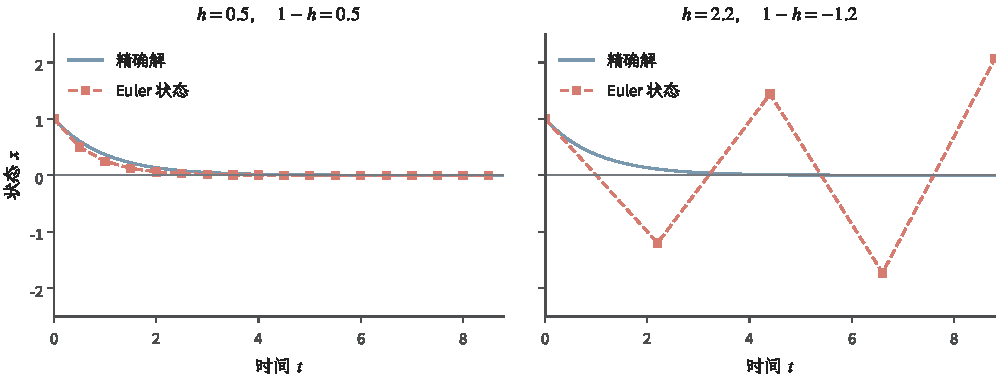
\includegraphics[width=\linewidth]{figures/math-preparation/dynamics/euler-stability.pdf}
  \caption{教学方程$\dot x=-x$、$x(0)=1$的精确解与Euler近似。蓝色实线是同一精确解，
  红色方点是各自步长下的数值状态；左图$h=0.5$衰减，右图$h=2.2$交替增长。
  两图使用相同坐标范围，连线仅显示相邻数值状态，不能解释为Euler方法在步间的精确解。}
  \label{fig:dynamical-euler-stability}
\end{figure*}

\subsection{仿射复合与前缀扫描}

轨迹的近似规则确定之后，还可改变同一递推的计算安排。前缀扫描同时求出从第一个更新起的
全部累计复合，例如$g_0$、$g_1\circ g_0$和$g_2\circ g_1\circ g_0$；它把相邻块先合并，
再逐层传播块结果，以减少串行依赖深度，数学上的时间顺序仍保持不变。考虑时变仿射递推
\begin{equation}
	\bm{x}_{k+1}= \bm{A}_{k}\bm{x}_{k}+\bm{b}_{k}. \label{eq:dynamical-affine-recurrence}
\end{equation}
把每一步表示为二元组 $g_{k}=(\bm{A}_{k},\bm{b}_{k})$，
并定义“后一步接在前一步之后”的组合
\begin{equation}
	(\bm{A}_{2},\bm{b}_{2}) \circ (\bm{A}_{1},\bm{b}_{1}) = (\bm{A}_{2}\bm{A}_{1},\,
	\bm{A}_{2}\bm{b}_{1}+\bm{b}_{2}). \label{eq:dynamical-affine-composition}
\end{equation}
直接展开三次复合可得
\[
	\begin{aligned}
	g_3\circ(g_2\circ g_1)
	&=(\bm{A}_3\bm{A}_2\bm{A}_1,\,
	\bm{A}_3\bm{A}_2\bm{b}_1+\bm{A}_3\bm{b}_2+\bm{b}_3)\\
	&=(g_3\circ g_2)\circ g_1,
	\end{aligned}
\]
所以该运算满足结合律。 由此，所有前缀 $g_{k-1}\circ\cdots\circ g_{0}$可以用并行前缀扫描组织，
再作用于$\bm{x}_{0}$得到每个状态。

结合律不等于交换律。 一般有
\[
	g_{2}\circ g_{1}\neq g_{1}\circ g_{2},
\]
因为矩阵乘法次序不同，偏置所经历的后续变换也不同。
例如令$g_1(\bm{x})=\operatorname{diag}(2,1)\bm{x}$，
$g_2(\bm{x})=\bm{x}+(1,0)^{\top}$。从$\bm{x}=\bm{0}$出发，
\[
	(g_2\circ g_1)(\bm{0})=(1,0)^{\top},\qquad
	(g_1\circ g_2)(\bm{0})=(2,0)^{\top}.
\]
同一个伸缩与平移只因交换次序就得到不同结果。
扫描算法可以改变括号位置以增加并行度， 不能改变时间顺序。
输入依赖或非线性更新若不形成封闭的结合运算，
也不能只因“看起来像递推”就使用同一扫描结构。

\section{判断扰动的长期衰减与短时放大}
\label{sec:dynamical-stability-sensitivity}

解的存在和数值计算都没有保证扰动会衰减。现在比较不同初值或输入产生的轨迹，
用谱与Lyapunov函数判断平衡点附近和较大区域内的长期行为。
原动力系统的稳定性与上节数值方法的稳定域必须分别检查，否则稳定方程也可能被步长算成发散递推。

\subsection{平衡点与稳定性}

一条轨迹最终靠近原点，不等于邻近初值在整个过程中都留在原点附近。稳定性比较的是
一组初值产生的全部正向轨迹，量词不能只落在选中的一个初值上。
\begin{definition}[平衡点与稳定性]
\label{def:dynamical-equilibrium-stability}
考虑局部Lipschitz自治系统$\dot{\bm{x}}=\bm{f}(\bm{x})$，下述稳定性均要求所涉及
初值的解对所有$t\geq0$存在。设$\bm{x}^{\star}$满足$\bm{f}(\bm{x}
^{\star})=\bm{0}$。 它称为平衡点。 平衡点在Lyapunov意义下\term{稳定}， 是指对每个$\varepsilon
>0$都存在$\delta>0$， 使$\lVert\bm{x}(0)-\bm{x}^{\star}\rVert <\delta$蕴含
\[
	\lVert\bm{x}(t)-\bm{x}^{\star}\rVert<\varepsilon \quad\text{对所有 }t\geq0.
\]
若它稳定，并且足够近的轨迹还满足 $\bm{x}(t)\to\bm{x}^{\star}$， 就称为\term{渐近稳定}。
若存在$r,C,\alpha>0$，使每个满足
$\lVert\bm{x}(0)-\bm{x}^{\star}\rVert_2<r$的初值都满足
\[
	\lVert\bm{x}(t)-\bm{x}^{\star}\rVert_2
	\leq C\mathrm{e}^{-\alpha t}
	\lVert\bm{x}(0)-\bm{x}^{\star}\rVert_2,
	\qquad t\geq0,
\]
则称该平衡点局部指数稳定。常数$C,\alpha$必须对这个邻域内的初值统一；
若同一界对任意初值成立，则称为全局指数稳定。
\end{definition}

稳定只要求轨迹不离开， 渐近稳定还要求轨迹回到平衡点。 系统$\dot{x}=0$的每个点都稳定，却没有一个孤立点吸引邻近轨迹。
稳定性也默认输入固定为所声明的值。 有外部输入时，需要另问有界输入产生多大状态响应，
不能把零输入稳定直接改写成任意输入下状态趋零。

三个稳定性概念可以在同一批标量方程上比较，见表~\ref{tab:dynamical-stability-types}。
指数条件中的统一常数决定了它比“最终回到原点”更强；不能对每个初值分别选一个
衰减率，再称为邻域上的指数稳定。

\begin{table*}[htbp]
  \centering
  \begin{tabularx}{\linewidth}{lXXX}
    \toprule
    方程与原点 & 小初值始终小 & 轨迹趋于原点 & 统一指数衰减\\
    \midrule
    $\dot x=0$ & 是，状态保持初值 & 否，非零初值不动 & 否\\
    $\dot x=-x^3$ & 是，$|x(t)|$不增 & 是，衰减为代数速度 & 否\\
    $\dot x=-x$ & 是 & 是 & 是，$|x(t)|=e^{-t}|x(0)|$\\
    \bottomrule
  \end{tabularx}
  \caption{零输入下的稳定、渐近稳定和指数稳定。第二行的解为
  $x(t)=x(0)/\sqrt{1+2x(0)^2t}$，说明吸引轨迹并不一定具有指数速度。三个例子均在
  全部$t\geq0$有解；表中比较的是相应方程原点的性质。}
  \label{tab:dynamical-stability-types}
\end{table*}

\subsection{线性系统的谱稳定判据}

对离散齐次系统
\begin{equation}
	\bm{x}_{k+1}=\bm{A}\bm{x}_{k}, \label{eq:dynamical-discrete-linear-homogeneous}
\end{equation}
有$\bm{x}_{k}=\bm{A}^{k}\bm{x}_{0}$。

\begin{theorem}[离散线性系统的渐近稳定性]
	\label{thm:dynamical-discrete-spectral-stability} 系统~\eqref{eq:dynamical-discrete-linear-homogeneous}的原点全局渐近稳定，
	当且仅当谱半径
	\[
		\rho(\bm{A}) = \max_{\lambda\in\operatorname{spec}(\bm{A})}|\lambda| <1.
	\]
\end{theorem}

\begin{proof}
	把$\bm{A}$在复数域写成Jordan形式 $\bm{A}=\bm{V}\bm{J}\bm{V}^{-1}$。 一个大小为$r$、特征值为$\lambda$的Jordan块满足
	\[
		\bm{J}_{\lambda}^{k}= \sum_{j=0}^{r-1}\binom{k}{j}\lambda^{k-j}\bm{N}^{j},
	\]
	其中$\bm{N}$为幂零矩阵。 若$|\lambda|<1$，多项式因子$k^{j}$仍被几何衰减压过，
	所以每个Jordan块趋零，进而$\bm{A}^{k}\to\bm{0}$。 这给出全局渐近稳定。

	反过来，若存在$|\lambda|>1$的特征值， 沿相应特征向量的状态会增长。 若$|\lambda|
	=1$， 沿普通特征向量的状态至少不趋零； 若相应Jordan块非平凡，还会出现多项式增长。
	因此渐近稳定要求全部特征值严格位于单位圆内。
\end{proof}

\begin{theorem}[连续线性系统的指数稳定性]
	\label{thm:dynamical-continuous-spectral-stability}
	连续线性系统$\dot{\bm{x}}=\bm{A}\bm{x}$的原点全局指数稳定，当且仅当
	$\bm{A}$的所有特征值实部严格为负。满足该条件的矩阵称为Hurwitz矩阵。
\end{theorem}

\begin{proof}
	对大小为$r$、特征值为$\lambda$的Jordan块，
	\[
		\mathrm{e}^{t(\lambda\bm{I}+\bm{N})}
		=\mathrm{e}^{\lambda t}\sum_{j=0}^{r-1}\frac{t^j}{j!}\bm{N}^j.
	\]
	若所有$\operatorname{Re}(\lambda)<0$，任选小于
	$-\max_\lambda\operatorname{Re}(\lambda)$的$\alpha>0$，
	各有限次多项式因子都可被$C\mathrm{e}^{-\alpha t}$控制。
	乘回换基矩阵后便有
	$\lVert\mathrm{e}^{t\bm{A}}\rVert\leq C\mathrm{e}^{-\alpha t}$，
	所以原点全局指数稳定。

	反过来，若某个特征值实部为正，沿对应实不变子空间存在指数增长的解；
	若实部为零，普通特征向量产生不衰减的振荡或常值解，非平凡Jordan块还会带来多项式增长。
	这些情形都不可能满足统一指数衰减界。
\end{proof}

离散系统检查单位圆，连续系统检查复平面的左半部；两者不能直接交换判据。

\subsection{Lyapunov函数与能量判据}

直接求解轨迹通常很难，但证明一个标量沿轨迹不增加可能容易得多。
\term{Lyapunov函数}（Lyapunov function）就是这样的偏离尺度；它不必等于物理能量。
\begin{definition}[Lyapunov函数]
\label{def:dynamical-lyapunov-function}
对原点为平衡点的自治系统$\dot{\bm x}=\bm f(\bm x)$，设$D$为原点的邻域。
若$V\in C^1(D)$满足$V(\bm0)=0$、$V(\bm x)>0$对所有非零$\bm x\in D$成立，
并且$\nabla V(\bm x)^\top\bm f(\bm x)\leq0$，则称$V$为该邻域内的Lyapunov函数。
若非零点处的最后一个不等式严格成立，则称它为严格Lyapunov函数。
\end{definition}
“正定”保证小能量确实表示靠近平衡点；“沿轨迹不增加”保证轨迹不能穿过更高的
能量边界。只有这两项合用，标量变化才能约束状态，而不是只约束某个可能忽略状态方向的指标。

下面的判据把这一思路落实为局部与全局稳定性条件\scite{math-khalil2002nonlinear}
\begin{theorem}[连续时间Lyapunov判据]
	\label{thm:dynamical-nonlinear-lyapunov} 设$\bm{x}^{\star}=\bm{0}$是 $\dot{\bm{x}}
=\bm{f}(\bm{x})$的平衡点，且$\bm{f}$在该点的某邻域内局部Lipschitz，使初值问题
具有唯一的最大解。若该邻域内存在连续可微函数$V$，满足
	\[
		V(\bm{0})=0,\qquad V(\bm{x})>0\quad(\bm{x}\neq\bm{0}),
	\]
	并且沿轨迹
	\[
		\dot V(\bm{x}) = \nabla V(\bm{x})^{\top}\bm{f}(\bm{x}) \leq0,
	\]
	则原点稳定。 若进一步对$\bm{x}\neq\bm{0}$有$\dot V(\bm{x})<0$，
则原点局部渐近稳定。若这些条件全局成立，$\bm{f}$在$\mathbb{R}^d$上局部Lipschitz，
且$V(\bm{x})\to\infty$随$\lVert\bm{x}\rVert\to\infty$成立，则所有最大解都可正向
延拓到任意时间，稳定性与吸引性为全局结论。
\end{theorem}

\begin{proof}
	固定一个足够小的$\varepsilon$， 使闭球包含在定理适用邻域内。 球面$\lVert\bm{x}\rVert
	=\varepsilon$是紧集， 而$V$在其上连续且正， 故最小值$c_{\varepsilon}>0$。 由$V(
	\bm{0})=0$与连续性， 可取$\delta>0$使 $\lVert\bm{x}(0)\rVert<\delta$蕴含
	$V(\bm{x}(0))<c_{\varepsilon}$。 由于$\dot V\leq0$， 轨迹不可能到达$V\geq c_{\varepsilon}$的球面，
	所以始终留在$\varepsilon$球内，得到稳定性。

	若$\dot V$负定，轨迹限制在一个紧的正子水平集$K$内。反设轨迹不趋近原点，
	则存在$\varepsilon_0>0$及趋向无穷的时刻序列，使
	$\lVert\bm{x}(t_j)\rVert\geq\varepsilon_0$。由于$\bm f$在$K$上有界，记
	$M=\sup_{\bm{x}\in K}\lVert\bm f(\bm{x})\rVert$；每次轨迹达到半径
	$\varepsilon_0$后，都至少在长度$\varepsilon_0/(2M)$的时间内留在闭环带
	$\varepsilon_0/2\leq\lVert\bm{x}\rVert\leq\sup_{\bm{z}\in K}\lVert\bm{z}\rVert$
	中。该环带紧且不含原点，连续函数$-\dot V$在其上有严格正的下界。选取互不相交
	的这些停留区间，$V$便会减少无穷大的总量，与$V\geq0$矛盾。因此轨迹趋向原点。
	径向无界性保证全局子水平集有界，轨迹无法在有限时间逃向无穷远，从而把同一论证
	扩展到任意初值。
\end{proof}

对线性系统，常取二次函数 $V(\bm{x})=\bm{x}^{\top}\bm{P}\bm{x}$。 沿$\dot{\bm{x}}=
\bm{A}\bm{x}$有
\begin{equation}
	\dot V(\bm{x}) = \bm{x}^{\top}(\bm{A}^{\top}\bm{P}+\bm{P}\bm{A}) \bm{x}. \label{eq:dynamical-continuous-lyapunov-derivative}
\end{equation}

\begin{theorem}[线性Lyapunov方程]
	\label{thm:dynamical-linear-lyapunov-equation} 矩阵$\bm{A}$为Hurwitz矩阵， 当且仅当对每个$\bm
	{Q}\succ\bm{0}$， 存在唯一$\bm{P}\succ\bm{0}$满足
	\begin{equation}
		\bm{A}^{\top}\bm{P}+\bm{P}\bm{A}= -\bm{Q}. \label{eq:dynamical-continuous-lyapunov-equation}
	\end{equation}
\end{theorem}

\begin{proof}
	若$\bm{A}$为Hurwitz矩阵，定义
	\[
		\bm{P}= \int_{0}^{\infty}\mathrm{e}^{t\bm{A}^{\top}}\bm{Q}\mathrm{e}^{t\bm{A}}
		\,\mathrm{d}t.
	\]
	指数稳定保证积分收敛。 对任意非零$\bm{x}$， 被积函数的二次型 $\lVert\bm{Q}^{1/2}
	\mathrm{e}^{t\bm{A}}\bm{x}\rVert_{2}^{2}$ 非负，并在$t=0$严格为正，所以$\bm{P}\succ
	\bm{0}$。 对被积矩阵求导并积分，
	\[
		\bm{A}^{\top}\bm{P}+\bm{P}\bm{A}= \left[ \mathrm{e}^{t\bm{A}^{\top}}\bm{Q}\mathrm{e}
		^{t\bm{A}}\right]_{0}^{\infty}= -\bm{Q}.
	\]
	唯一性可由齐次方程 $\bm{A}^{\top}\bm{D}+\bm{D}\bm{A}=\bm{0}$ 沿流积分得到$\bm{D}
	=\bm{0}$。

	反过来，若存在$\bm{P},\bm{Q}\succ\bm{0}$满足该方程， 式~\eqref{eq:dynamical-continuous-lyapunov-derivative}给出
	$\dot V=-\bm{x}^{\top}\bm{Q}\bm{x}<0$。 Lyapunov判据推出原点渐近稳定， 线性系统因而要求$\bm
	{A}$全部特征值实部为负。
\end{proof}

离散时间对应方程为
\[
	\bm{A}^{\top}\bm{P}\bm{A}-\bm{P}= -\bm{Q}.
\]
它检验一步前后能量差， 与连续时间方程的导数形式不同。

\begin{theorem}[离散时间Lyapunov方程]
	\label{thm:dynamical-discrete-lyapunov-equation}
	离散线性系统$\bm{x}_{k+1}=\bm{A}\bm{x}_k$满足$\rho(\bm{A})<1$，当且仅当对每个
	$\bm{Q}\succ\bm{0}$，存在唯一$\bm{P}\succ\bm{0}$满足
	\[
		\bm{A}^{\top}\bm{P}\bm{A}-\bm{P}=-\bm{Q}.
	\]
\end{theorem}

\begin{proof}
	若$\rho(\bm{A})<1$，定义
	\[
		\bm{P}=\sum_{j=0}^{\infty}(\bm{A}^{\top})^j\bm{Q}\bm{A}^j.
	\]
	定理~\ref{thm:dynamical-discrete-spectral-stability}及有限维范数等价性保证级数收敛。
	其首项为$\bm{Q}\succ\bm{0}$，其余项半正定，所以$\bm{P}\succ\bm{0}$。
	将级数左乘$\bm{A}^{\top}$、右乘$\bm{A}$后与原式相减，便得到Lyapunov方程。
	若$\bm{P}_1,\bm{P}_2$都是解，令$\bm{D}=\bm{P}_1-\bm{P}_2$，则
	$\bm{D}=(\bm{A}^{\top})^k\bm{D}\bm{A}^k$；令$k\to\infty$即得$\bm{D}=\bm{0}$。

	反过来，若存在$\bm{P},\bm{Q}\succ\bm{0}$满足方程，则
	\[
		V(\bm{x}_{k+1})-V(\bm{x}_k)
		=-\bm{x}_k^{\top}\bm{Q}\bm{x}_k,
		\qquad V(\bm{x})=\bm{x}^{\top}\bm{P}\bm{x}.
	\]
	由紧单位球上
	$\bm{x}^{\top}\bm{A}^{\top}\bm{P}\bm{A}\bm{x}/(\bm{x}^{\top}\bm{P}\bm{x})<1$
	取得统一上界$c<1$，故$V(\bm{x}_k)\leq c^kV(\bm{x}_0)$。
	原点指数稳定，定理~\ref{thm:dynamical-discrete-spectral-stability}于是给出$\rho(\bm{A})<1$。
\end{proof}

\subsection{LaSalle不变性与极限集}

严格负的$\dot V$迫使轨迹离开每个非平衡状态；只有$\dot V\leq0$时，轨迹却可能停留或运动在
零导数集合中。要区分这两种情况，需要描述系统长期能够留在哪些状态。
\begin{definition}[不变集合与轨迹极限集]
\label{def:dynamical-invariant-limit-sets}
设自治向量场局部Lipschitz，$\Phi_t$为其唯一解生成的流。以下集合上的解须在所有$t\geq0$存在。
集合$\Omega$称为\term{正向不变集}（positively invariant set），若从任意
$\bm{x}_0\in\Omega$出发的解在所有后续存在时刻都留在$\Omega$。
对自治系统记正向流为$\Phi_t$。集合$M$称为\term{不变集}（invariant set），若对
每个$t\geq0$都有$\Phi_t(M)=M$。等号比正向不变所要求的
$\Phi_t(M)\subseteq M$更强：它还要求$M$中的每一点都能在$M$内找到任意时长以前的
前像；等价地，每一点都位于一条始终留在$M$中的完整轨迹上。
一条正向有界轨迹$\bm{x}(t)$的\term{$\omega$极限集}定义为
\[
	\omega(\bm{x}_0)
	=\left\{\bm{z}:\ \text{存在 }t_j\to\infty
	\text{ 使 }\bm{x}(t_j)\to\bm{z}\right\}.
\]
\end{definition}
正向不变集约束从集合中每一点出发的整段未来；$\omega$极限集则记录一条轨迹在无限远时间反复接近的状态。

\begin{theorem}[LaSalle不变性原理]
	\label{thm:dynamical-lasalle-invariance}
	设自治系统$\dot{\bm{x}}=\bm{f}(\bm{x})$的向量场局部Lipschitz，
	$\Omega$是紧的正向不变集，$V$在包含$\Omega$的开邻域上连续可微，且
	$\dot V(\bm{x})=\nabla V(\bm{x})^{\top}\bm{f}(\bm{x})\leq0$。
	记$E=\{\bm{x}\in\Omega:\dot V(\bm{x})=0\}$，并令$M$为包含在$E$中的最大不变集。
	则每条从$\Omega$出发的轨迹都满足
	\[
		\operatorname{dist}(\bm{x}(t),M)\longrightarrow0.
	\]
\end{theorem}

\begin{proof}
	紧性和正向不变性使轨迹正向预紧，并排除有限时间逃逸，所以
	$\omega(\bm{x}_0)$非空且紧。函数$t\mapsto V(\bm{x}(t))$单调不增并有下界，
	因而收敛到某个$v_{\infty}$。若$\bm{z}\in\omega(\bm{x}_0)$，
	取$t_j\to\infty$使$\bm{x}(t_j)\to\bm{z}$，连续性给出$V(\bm{z})=v_{\infty}$。

	还要核对这里需要的是不变，而不只是正向不变。自治流对初值连续。对任意固定
	$s\geq0$，$\bm{x}(t_j+s)\to\Phi_s(\bm{z})$，所以
	$\Phi_s(\bm{z})\in\omega(\bm{x}_0)$，得到
	$\Phi_s(\omega(\bm{x}_0))\subseteq\omega(\bm{x}_0)$。反过来，对充分大的$j$考察
	$\bm{x}(t_j-s)$；紧性允许取子列使其收敛到某个
	$\bm{w}\in\omega(\bm{x}_0)$，而流的连续性给出
	$\Phi_s(\bm{w})=\bm{z}$。因此
	$\Phi_s(\omega(\bm{x}_0))=\omega(\bm{x}_0)$，极限集确实是不变集。

	函数$V$在$\omega(\bm{x}_0)$上恒为$v_{\infty}$。从其中任一点出发的轨迹仍留在
	该极限集，沿轨迹求导便有$\dot V=0$。于是
	$\omega(\bm{x}_0)$是$E$中的不变集，故
	$\omega(\bm{x}_0)\subseteq M$。

	还需把极限点结论转成整条尾轨迹的距离结论。若
	$\operatorname{dist}(\bm{x}(t),M)$不趋零，就存在$\varepsilon>0$和$t_j\to\infty$
	使这些距离至少为$\varepsilon$。紧性允许取收敛子列，其极限属于
	$\omega(\bm{x}_0)\subseteq M$，与距离下界矛盾。
\end{proof}

\begin{example}[阻尼振子的零导数集合]
	\label{ex:dynamical-damped-oscillator-lasalle}
	考虑
	\[
		\dot q=p,\qquad \dot p=-q-cp,\qquad c>0,
	\]
	并取$V(q,p)=(q^2+p^2)/2$。沿轨迹
	\[
		\dot V=q\dot q+p\dot p=-cp^2\leq0.
	\]
	零导数集合是整条直线$E=\{(q,p):p=0\}$，但其中$q\neq0$的点满足
	$\dot p=-q\neq0$，会立刻离开$E$。因此$E$中的最大不变子集只有原点。
	任意能量子水平集都紧且正向不变，定理~\ref{thm:dynamical-lasalle-invariance}
	遂说明所有轨迹趋向原点。仅由“$p=0$时能量瞬间不变”不能得到同一结论。
\end{example}

图~\ref{fig:reader-lasalle-zero-set}取$c=1$并从$(q,p)=(1,0)$出发。
起点虽然位于$\dot V=0$的直线上，速度$(0,-1)$却指向直线之外；随后轨迹绕原点衰减。
LaSalle需要的是能一直留在零导数集合中的完整轨迹，而不是某一瞬间导数恰为零的点。
\begin{figure}[htbp]
  \centering
  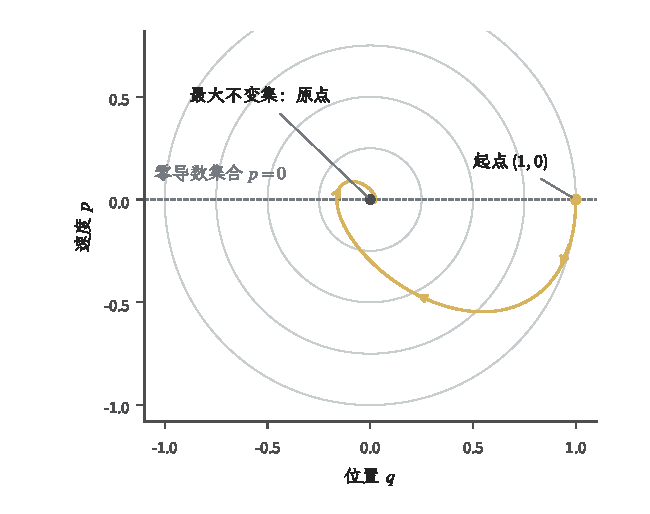
\includegraphics[width=\linewidth]{figures/math-preparation/reader-revision-dynamics/lasalle-zero-set.pdf}
  \caption{教学阻尼振子$\dot q=p$、$\dot p=-q-p$的精确轨迹，初态$(1,0)$。
  黄色轨迹在$t=0$至$12$间逐渐靠近原点，箭头表示时间前进；灰色虚线是零导数集合$p=0$，
  浅灰圆是$V=(q^2+p^2)/2$的参考等值线。整条零导数直线并不不变，原点才是其中最大不变集。}
  \label{fig:reader-lasalle-zero-set}
\end{figure}


\subsection{非正规动态与瞬态放大}

谱只决定渐近指数率，不保证每一步都缩小欧氏范数。考虑离散系统
\[
	\bm{A}=
	\begin{bmatrix}
		1/2 & K  \\
		0   & 1/2
	\end{bmatrix}, \qquad K>0.
\]
两个特征值都等于$1/2$，所以$\rho(\bm{A})<1$。然而
\[
	\bm{A}^k=
	\begin{bmatrix}
		2^{-k} & kK\,2^{-(k-1)} \\
		0      & 2^{-k}
	\end{bmatrix}.
\]
从$\bm{x}_{0}=(0,1)^{\top}$出发，第一步状态为$(K,1/2)^{\top}$；
当$K$很大时，欧氏范数立刻远大于初始范数，随后才因$k2^{-k}\to0$而衰减。

图~\ref{fig:dynamical-transient-growth}取$K=4$，与$K=0$的同谱系统比较。
非零耦合把第二个坐标中的初始扰动传入第一个坐标，造成短时放大；两者的特征值
完全相同，后期也都衰减。因而谱条件不能替代“每一步状态范数都缩小”的判断。
\begin{figure}[htbp]
  \centering
  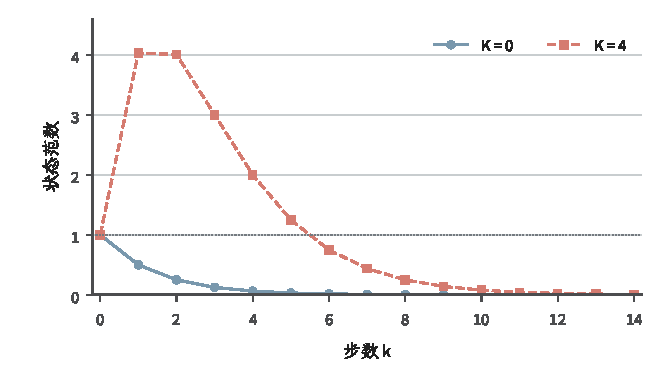
\includegraphics[width=\linewidth]{figures/math-preparation/concept-revision-dynamics/transient-growth.pdf}
  \caption{离散教学系统$\bm A=\left[\begin{smallmatrix}1/2&K\\0&1/2\end{smallmatrix}\right]$
  从$\bm x_0=(0,1)^\top$出发。蓝色圆点取$K=0$，红色方点取$K=4$；两者谱半径均为$1/2$。
  后者在前两步的欧氏范数约为$4.03$、$4.01$，然后趋零。灰线标记初始范数$1$，
  图中放大来自状态耦合，未加入输入或数值离散误差。}
  \label{fig:dynamical-transient-growth}
\end{figure}

这种现象来自矩阵非正规，即$\bm{A}^{\top}\bm{A}\neq\bm{A}\bm{A}^{\top}$。
在当前例子中，$\bm{A}=\tfrac12\bm{I}+\bm{N}$且$\bm{N}^2=\bm{0}$；
$K\neq0$时矩阵只有一个线性无关的特征向量，广义特征向量链的幂零耦合产生了
$k2^{-k}$因子。可对角化的非正规矩阵还可能通过近乎共线的特征向量，使不同衰减率的模态
先相消、后解消，从而产生另一类瞬态放大。因此，长期谱结论不能替代有限时间增益、
伪谱或合适Lyapunov范数的分析。

\subsection{初值敏感性与输入扰动响应}

若$\bm{f}$关于状态具有Lipschitz常数$L$， 两条使用同一输入的解满足
\[
	\lVert\bm{x}(t)-\widetilde{\bm{x}}(t)\rVert \leq \mathrm{e}^{L(t-t_0)}\lVert\bm
	{x}_{0}-\widetilde{\bm{x}}_{0}\rVert.
\]
这是Gronwall不等式给出的有限时间敏感性上界。 它保证连续依赖于初值， 却在$L>0$时不表示扰动衰减。

对指数稳定线性系统， 若存在$M,\alpha>0$使
$\lVert\mathrm{e}^{t\bm{A}}\rVert\leq M \mathrm{e}^{-\alpha t}$， 则式~\eqref{eq:dynamical-lti-variation-constants}给出
\[
	\lVert\bm{x}(t)\rVert \leq M\mathrm{e}^{-\alpha(t-t_0)}\lVert\bm{x}_{0}\rVert+ M
	\lVert\bm{B}\rVert \int_{t_0}^{t}\mathrm{e}^{-\alpha(t-s)}\lVert\bm{u}(s)\rVert
	\,\mathrm{d}s.
\]
有界输入因而产生有界状态， 但状态一般不会趋零。 输入、初值与模型扰动是不同来源， 稳定性结论应说明控制的是哪一种。

\section{由观测历史估计隐藏状态}
\label{sec:dynamical-stochastic-state-observation}

到这里，初值和输入给定后主要考察确定性轨迹。恢复过程噪声后，状态成为随机变量，
只能观察带噪输出时，还需区分状态分布与给定观测历史的条件分布。
本节先建立预测核和观测核，下一节才在高斯闭合条件下计算具体的滤波和平滑递推。

\subsection{用转移核与观测核表示未知状态}

恢复式~\eqref{eq:dynamical-linear-state-model}与 \eqref{eq:dynamical-linear-observation-model}中的噪声。
过程噪声$\bm{w}_{k}$直接进入状态演化， 表示模型没有显式描述的随机作用； 观测噪声$\bm
{v}_{k}$只污染读数， 不直接改变真实状态。 即使二者最终都使估计不确定，
它们在联合分布中的位置不同。

给定初始分布和输入序列， 状态转移核为
\[
	K_{k}(\bm{x},A) = \mathbb{P}\!\left( \bm{A}_{k}\bm{x}+\bm{B}_{k}\bm{u}_{k}+\bm{w}
	_{k}\in A \right).
\]
在标准加性状态空间模型中，先假设初值、各时刻过程噪声以及各时刻观测噪声相互独立，
输入序列为给定量。于是$\bm{w}_k$在给定$\bm{x}_k$后，与
$\sigma(\bm{x}_{0:k-1},\bm{y}_{1:k},\bm{u}_{0:k})$条件独立，状态过程满足
条件Markov性质
\[
	\mathbb{P}( \bm{x}_{k+1}\in A \mid \bm{x}_{0:k},\bm{y}_{1:k},\bm{u}_{0:k}) = K_{k}
	(\bm{x}_{k},A).
\]
Markov性质针对真实状态。 观测序列自身通常不是Markov链， 因为当前观测未必包含预测下一观测所需的全部状态信息。

与状态转移核相对，观测核
\[
	G_k(\bm{x},B)
	=\mathbb{P}(\bm{y}_k\in B\mid \bm{x}_k=\bm{x})
\]
规定给定当前状态后会看到什么。在标准状态空间模型中，给定$\bm{x}_k$以后，
$\bm{y}_k$与更早的状态、观测和噪声条件独立。若过程噪声与观测噪声相关，
或者传感器还直接依赖旧状态，就必须把相关变量并入联合状态或显式修改这个条件独立结构。

记$\mathcal{Y}_{k}=\sigma(\bm{y}_{1},\ldots,\bm{y}_{k})$。在只观察$\bm{y}$时，
可用于预测未来的对象变成状态的条件分布。
\begin{definition}[滤波分布]
\label{def:dynamical-filtering-distribution}
对标准状态空间模型中的欧氏状态和观测，给定$\mathcal Y_k$后的状态条件概率核
\begin{equation}
	\pi_{k}(A) = \mathbb{P}(\bm{x}_{k}\in A\mid\mathcal{Y}_{k}), \label{eq:dynamical-filtering-distribution}
\end{equation}
称为\term{滤波分布}（filtering distribution），其中$A$遍历状态空间的Borel集合。
\end{definition}
它是根据截至当前的观测对隐藏状态形成的条件分布。
真实状态$\bm{x}_{k}$、带噪读数$\bm{y}_{k}$与条件分布$\pi_{k}$
分别是潜在对象、数据和推断结果，不能用同一个“状态”含混指代。

信息不足即使没有观测噪声也可能出现。例如$\bm{x}_k=(x_{1,k},x_{2,k})^{\top}$，
而传感器只返回$y_k=x_{1,k}+x_{2,k}$。观测$y_k=1$不能区分
$(1,0)^{\top}$与$(0,1)^{\top}$；动力学和后续观测或许能逐步区分这两个方向，
但这需要额外结构。第~\ref{chap:control-theory}章将用可观测性和可检测性精确刻画线性系统中哪些方向可以恢复。

\subsection{先传播预测，再用新证据校正}

设当前滤波分布为$\pi_{k-1}$。 先通过状态转移核得到预测分布
\begin{equation}
	\pi_{k\mid k-1}(A) = \int K_{k-1}(\bm{x},A) \,\pi_{k-1}(\mathrm{d}\bm{x}). \label{eq:dynamical-general-prediction-kernel}
\end{equation}
要把校正写成密度形式，还需假设存在与状态$\bm{x}$无关的共同$\sigma$有限支配测度
$\nu_k$以及联合可测函数$g_k$，使
\[
	G_k(\bm{x},\mathrm{d}\bm{y})
	=g_k(\bm{y}\mid\bm{x})\nu_k(\mathrm{d}\bm{y}).
\]
观测$\bm{y}_{k}$到来后，再用似然密度
$g_{k}(\bm{y}_{k}\mid\bm{x}_{k})$重新加权：
\begin{equation}
	\pi_{k}(\mathrm{d}\bm{x}) =
	\frac{g_{k}(\bm{y}_{k}\mid\bm{x})\pi_{k\mid k-1}(\mathrm{d}\bm{x})}
	{\int g_{k}(\bm{y}_{k}\mid\bm{z})\pi_{k\mid k-1}(\mathrm{d}\bm{z})}. \label{eq:dynamical-general-bayes-filter}
\end{equation}
这个公式适用于分母有限且严格为正的观测值。预测传播动力学不确定性，
校正利用新观测改变相对权重；两步分别来自全概率公式和Bayes公式。

\begin{example}[两状态模型的一次预测与校正]
	\label{ex:dynamical-two-state-bayes-filter}
	设隐藏状态取值于$\{0,1\}$，当前滤波概率为
	$\pi_0(0)=0.7$、$\pi_0(1)=0.3$，转移矩阵按“当前状态为行、下一状态为列”写成
	\[
		\bm{P}=
		\begin{bmatrix}
			0.8 & 0.2\\
			0.1 & 0.9
		\end{bmatrix}.
	\]
	一步预测得到
	\[
		\pi_{1\mid0}(1)=0.7\times0.2+0.3\times0.9=0.41,\qquad
		\pi_{1\mid0}(0)=0.59.
	\]
	再设观测$y_1\in\{0,1\}$满足
	$\mathbb{P}(y_1=1\mid x_1=0)=0.2$、
	$\mathbb{P}(y_1=1\mid x_1=1)=0.8$。实际看到$y_1=1$后，
	\[
		\pi_1(1)
		=\frac{0.8\times0.41}{0.2\times0.59+0.8\times0.41}
		=\frac{164}{223}\approx0.735.
	\]
	预测步骤把上一时刻的不确定性穿过转移矩阵，校正步骤才用观测似然重新分配概率。
	整个计算只保存$\pi_0$而不保存更早观测，正是因为标准条件独立结构已经把过去信息压缩进当前滤波分布。
\end{example}

\begin{example}[带泄漏温度的间接观测]
	\label{ex:dynamical-noisy-temperature} 设房间相对环境的温差满足
	\[
		x_{k+1}=0.9x_{k}+u_{k}+w_{k}, \qquad y_{k}=x_{k}+v_{k}.
	\]
	即使$v_{k}=0$，未来温差仍因$w_{k}$不确定； 即使$w_{k}=0$，当前温差仍不能从带噪$y
	_{k}$精确知道。 若两种噪声同时存在， 预测阶段因过程噪声扩大不确定性， 校正阶段再根据传感器精度缩小不确定性。
	把$y_{k}$直接当作$x_{k}$会忽略观测噪声， 只按确定递推外推又会忽略过程噪声。
\end{example}

\subsection{在线性高斯模型中封闭分布递推}
\label{sec:dynamical-kalman-rts}

为了得到解析递推，下面采用有限时域线性高斯模型：
\begin{align*}
	\bm{x}_{0} & \sim \mathcal{N}(\bm{m}_{0\mid0},\bm{P}_{0\mid0}), \\
	\bm{w}_{k} & \sim \mathcal{N}(\bm{0},\bm{\Sigma}_{\mathrm{w},k}),               \\
	\bm{v}_{k} & \sim \mathcal{N}(\bm{0},\bm{\Sigma}_{\mathrm{v},k}).
\end{align*}
假设初值、全部过程噪声和全部观测噪声彼此独立，输入与系统矩阵为给定量。允许
$\bm{\Sigma}_{\mathrm{w},k}$半正定，并先假设
$\bm{\Sigma}_{\mathrm{v},k}\succ\bm{0}$，以保证后续创新协方差可逆。

线性变换保持高斯性， 联合高斯的条件分布仍为高斯。 因此只需递推条件均值与条件协方差，
便能完整表示每个滤波分布。 若初值或噪声非高斯， 均值和协方差更新仍可能给出最佳线性估计，
却不再完整描述条件分布，也不能无条件称为精确Bayes滤波。

高斯性使整个分布可以由均值与协方差保存，但递推以前仍须先固定允许使用哪一段观测。

\subsubsection{预测、滤波与平滑的信息条件}

记
\begin{align*}
	\bm{m}_{k\mid j} & := \mathbb{E}[\bm{x}_{k}\mid\mathcal{Y}_{j}],         \\
	\bm{P}_{k\mid j} & := \operatorname{Cov}(\bm{x}_{k}\mid\mathcal{Y}_{j}).
\end{align*}
一步预测使用$\mathcal{Y}_{k-1}$估计$\bm{x}_{k}$， 滤波使用$\mathcal{Y}_{k}$估计同一当前状态，
平滑则在固定终点$T>k$后使用$\mathcal{Y}_{T}$重新估计过去状态。
未来观测能够帮助平滑， 因为它们包含过去状态经过动力学传播后的信息。

表~\ref{tab:dynamical-estimation-information}固定同一个目标$x_k$，只改变允许使用的
观测。区别在信息集合，而不在是否使用某一种算法。在线决策到时刻$k$只能调用前两行；
把事后平滑结果当作在线估计，会让当前决策使用尚未发生的观测。

\begin{table}[htbp]
  \centering
  \begin{tabularx}{\linewidth}{lXX}
    \toprule
    推断 & 条件分布 & 可用观测\\
    \midrule
    一步预测 & $P(\bm{x}_k\mid\mathcal Y_{k-1})$ & 新读数到来之前的历史\\
    当前滤波 & $P(\bm{x}_k\mid\mathcal Y_k)$ & 截至当前的新旧读数\\
    固定区间平滑 & $P(\bm{x}_k\mid\mathcal Y_T)$，$T>k$ & 事后取得的未来读数\\
    \bottomrule
  \end{tabularx}
  \caption{预测、滤波与平滑针对同一状态，却允许使用不同信息。向量状态的条件分布采用
  同样的口径，$\mathcal Y_j$表示截至时刻$j$的观测所生成的信息。}
  \label{tab:dynamical-estimation-information}
\end{table}

\subsubsection{预测均值与协方差传播}

假设
\[
	\bm{x}_{k-1}\mid\mathcal{Y}_{k-1}\sim \mathcal{N}( \bm{m}_{k-1\mid k-1}, \bm{P}
	_{k-1\mid k-1}).
\]
由状态方程和独立零均值过程噪声，
\begin{align}
	\bm{m}_{k\mid k-1} & = \bm{A}_{k-1}\bm{m}_{k-1\mid k-1}+\bm{B}_{k-1}\bm{u}_{k-1}, \label{eq:dynamical-kalman-predicted-mean}              \\
	\bm{P}_{k\mid k-1} & = \bm{A}_{k-1}\bm{P}_{k-1\mid k-1}\bm{A}_{k-1}^{\top}+\bm{\Sigma}_{\mathrm{w},k-1}. \label{eq:dynamical-kalman-predicted-covariance}
\end{align}
交叉协方差项消失的依据是 $\bm{w}_{k-1}$与 $\bm{x}_{k-1}\mid\mathcal{Y}_{k-1}$独立且均值为零。
若过程噪声与旧状态相关， 式~\eqref{eq:dynamical-kalman-predicted-covariance} 还要保留相应交叉项。

\subsubsection{条件高斯更新与Kalman滤波}

给定$\mathcal{Y}_{k-1}$， 预测状态与新观测的联合分布为
\begin{equation}
	\begin{bmatrix}
		\bm{x}_{k} \\
		\bm{y}_{k}
	\end{bmatrix}
	\Biggm|\mathcal{Y}_{k-1}\sim \mathcal{N}\left(
	\begin{bmatrix}
		\bm{m}_{k\mid k-1}           \\
		\bm{C}_{k}\bm{m}_{k\mid k-1}
	\end{bmatrix},
	\begin{bmatrix}
		\bm{P}_{k\mid k-1}           & \bm{P}_{k\mid k-1}\bm{C}_{k}^{\top} \\
		\bm{C}_{k}\bm{P}_{k\mid k-1} & \bm{S}_{k}
	\end{bmatrix}
	\right), \label{eq:dynamical-kalman-joint-gaussian}
\end{equation}
其中
\begin{equation}
	\bm{S}_{k}= \bm{C}_{k}\bm{P}_{k\mid k-1}\bm{C}_{k}^{\top}+\bm{\Sigma}_{\mathrm{v},k}\label{eq:dynamical-kalman-innovation-covariance}
\end{equation}
是\term{创新协方差}，
\[
	\bm{r}_{k}= \bm{y}_{k}-\bm{C}_{k}\bm{m}_{k\mid k-1}
\]
是创新，即新观测超出预测观测的部分。

由于$\bm{\Sigma}_{\mathrm{v},k}\succ\bm{0}$， 有$\bm{S}_{k}\succ\bm{0}$并可逆。 把第~\ref{sec:probability-random-vectors-transformations}节的
条件高斯公式用于联合分布~\eqref{eq:dynamical-kalman-joint-gaussian}， 得到
\begin{align}
	\bm{K}_{k}       & = \bm{P}_{k\mid k-1}\bm{C}_{k}^{\top}\bm{S}_{k}^{-1}, \label{eq:dynamical-kalman-gain}                       \\
	\bm{m}_{k\mid k} & = \bm{m}_{k\mid k-1}+\bm{K}_{k}\bm{r}_{k}, \label{eq:dynamical-kalman-filtered-mean}                         \\
	\bm{P}_{k\mid k} & = \bm{P}_{k\mid k-1}- \bm{K}_{k}\bm{S}_{k}\bm{K}_{k}^{\top}. \label{eq:dynamical-kalman-filtered-covariance}
\end{align}
式~\eqref{eq:dynamical-kalman-gain}中的 $\bm{K}_{k}$称为Kalman增益。 它不是手工设定的学习率，
而是预测误差与观测误差协方差共同决定的条件高斯系数
\scite{math-kalman1960filtering}

\begin{theorem}[有限时域Kalman滤波]
	\label{thm:dynamical-finite-horizon-kalman-filter} 在本节线性高斯初值、独立高斯噪声及
	$\bm{S}_{k}$可逆的条件下， 递推~\eqref{eq:dynamical-kalman-predicted-mean}至
	\eqref{eq:dynamical-kalman-filtered-covariance} 精确给出
	\[
		\bm{x}_{k}\mid\mathcal{Y}_{k}\sim \mathcal{N}( \bm{m}_{k\mid k}, \bm{P}_{k\mid
		k})
	\]
	对每个有限$k$成立。
\end{theorem}

\begin{proof}
	对$k$归纳。 初值按假设为高斯。 若$\bm{x}_{k-1}\mid\mathcal{Y}_{k-1}$为高斯，
	线性状态方程与独立高斯过程噪声使 $\bm{x}_{k}\mid\mathcal{Y}_{k-1}$仍为高斯，
	其均值和协方差由 \eqref{eq:dynamical-kalman-predicted-mean}与 \eqref{eq:dynamical-kalman-predicted-covariance}给出。
	观测又是预测状态与独立高斯噪声的线性组合， 所以联合分布为 \eqref{eq:dynamical-kalman-joint-gaussian}。
	条件高斯公式给出 \eqref{eq:dynamical-kalman-filtered-mean}与 \eqref{eq:dynamical-kalman-filtered-covariance}，
	完成归纳。
\end{proof}

协方差更新还可写成Joseph形式
\begin{equation}
	\bm{P}_{k\mid k}= (\bm{I}-\bm{K}_{k}\bm{C}_{k}) \bm{P}_{k\mid k-1}(\bm{I}-\bm{K}
	_{k}\bm{C}_{k})^{\top}+ \bm{K}_{k}\bm{\Sigma}_{\mathrm{v},k}\bm{K}_{k}^{\top}. \label{eq:dynamical-kalman-joseph-form}
\end{equation}
代入Kalman增益并展开，可化为 式~\eqref{eq:dynamical-kalman-filtered-covariance}。
Joseph形式把两类误差来源都写成半正定项，
在有限精度实现中更容易维持协方差的对称与半正定。 实现时也应通过线性求解获得
$\bm{S}_{k}^{-1}\bm{r}_{k}$， 而不是显式形成逆矩阵。

\begin{example}[标量观测怎样权衡预测与读数]
	\label{ex:dynamical-scalar-kalman-update} 若预测方差为$p^{-}$，观测为$y=x+v$， 且$v
	\sim\mathcal{N}(0,r)$，则
	\[
		K=\frac{p^{-}}{p^{-}+r}, \qquad m^{+}=m^{-}+K(y-m^{-}), \qquad
		p^{+}=\frac{p^{-}r}{p^{-}+r}.
	\]
	当$r$很小，增益接近$1$，更新更相信读数； 当$r$很大，增益接近$0$，更新更相信预测。
	即使$r\to0$， 只有被直接观测的方向会被精确校正； 多维系统中未被$\bm{C}_{k}$区分的方向仍可能保留不确定性。

	例如$m^-=0$、$p^-=4$、$r=1$且实际读数$y=2$时，
	\[
		K=\frac45,\qquad m^+=\frac85,\qquad p^+=\frac45.
	\]
	后验均值位于预测均值$0$与读数$2$之间，后验方差也小于预测方差和观测噪声方差；
	后一比较依赖两项误差独立且方差均为正。
\end{example}

图~\ref{fig:dynamical-kalman-density-update}展示刚才的标量计算。后验向读数移动，同时
变窄，因为独立的新读数排除了部分原本可能的状态。密度曲线的纵轴是密度而非单点概率，
曲线变高表示质量集中，曲线下的总面积仍为$1$。这个几何解释只适用于此处的高斯、
独立噪声设定；观测值与预测不一致，并不总意味着真实过程本身发生了跳变。

\begin{figure}[htbp]
  \centering
  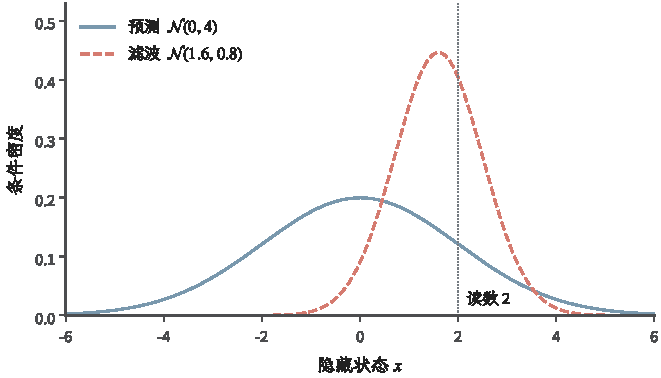
\includegraphics[width=\linewidth]{figures/math-preparation/dynamics/kalman-density-update.pdf}
  \caption{标量Kalman更新的教学例。蓝色曲线为预测$\mathcal N(0,4)$，红色曲线为观察
  $y=2$后得到的$\mathcal N(1.6,0.8)$，观测噪声方差为$1$，虚线标记实际读数。
  这里$\mathcal N$的第二个参数是方差；比较的是同一隐藏状态在新观测前后的条件密度。}
  \label{fig:dynamical-kalman-density-update}
\end{figure}

\subsection{利用未来观测修正过去状态}

滤波只向前传递。 固定终点$T$后， Rauch--Tung--Striebel（RTS）平滑器从 $k=T-1$向后计算
$p(\bm{x}_{k}\mid\mathcal{Y}_{T})$\scite{math-rauch1965smoothing} 关键是先求
$p(\bm{x}_{k}\mid\bm{x}_{k+1},\mathcal{Y}_{k})$。

给定$\mathcal{Y}_{k}$， 由状态方程可得联合高斯
\[
	\begin{bmatrix}
		\bm{x}_{k}   \\
		\bm{x}_{k+1}
	\end{bmatrix}
	\Biggm|\mathcal{Y}_{k}\sim \mathcal{N}\left(
	\begin{bmatrix}
		\bm{m}_{k\mid k}   \\
		\bm{m}_{k+1\mid k}
	\end{bmatrix},
	\begin{bmatrix}
		\bm{P}_{k\mid k}           & \bm{P}_{k\mid k}\bm{A}_{k}^{\top} \\
		\bm{A}_{k}\bm{P}_{k\mid k} & \bm{P}_{k+1\mid k}
	\end{bmatrix}
	\right).
\]
若$\bm{P}_{k+1\mid k}$可逆， 条件高斯公式给出
\begin{align}
	\bm{J}_{k}                                                       & = \bm{P}_{k\mid k}\bm{A}_{k}^{\top}\bm{P}_{k+1\mid k}^{-1}, \label{eq:dynamical-rts-gain}                                   \\
	\mathbb{E}[ \bm{x}_{k}\mid \bm{x}_{k+1},\mathcal{Y}_{k}]         & = \bm{m}_{k\mid k}+ \bm{J}_{k}(\bm{x}_{k+1}-\bm{m}_{k+1\mid k}), \label{eq:dynamical-rts-one-step-conditional-mean}         \\
	\operatorname{Cov}( \bm{x}_{k}\mid \bm{x}_{k+1},\mathcal{Y}_{k}) & = \bm{P}_{k\mid k}- \bm{J}_{k}\bm{P}_{k+1\mid k}\bm{J}_{k}^{\top}. \label{eq:dynamical-rts-one-step-conditional-covariance}
\end{align}

\begin{theorem}[有限时域RTS平滑]
	\label{thm:dynamical-rts-smoother} 在有限时域Kalman滤波条件下， 并假设每个$\bm{P}
	_{k+1\mid k}$可逆， 以
	\[
		\bm{m}_{T\mid T},\qquad \bm{P}_{T\mid T}
	\]
	为终点，向后递推
	\begin{align}
		\bm{m}_{k\mid T} & = \bm{m}_{k\mid k}+ \bm{J}_{k}(\bm{m}_{k+1\mid T}-\bm{m}_{k+1\mid k}), \label{eq:dynamical-rts-smoothed-mean}                       \\
		\bm{P}_{k\mid T} & = \bm{P}_{k\mid k}+ \bm{J}_{k}(\bm{P}_{k+1\mid T}-\bm{P}_{k+1\mid k}) \bm{J}_{k}^{\top}\label{eq:dynamical-rts-smoothed-covariance}
	\end{align}
	可精确得到 $\bm{x}_{k}\mid\mathcal{Y}_{T}$的均值与协方差。
\end{theorem}

\begin{proof}
	状态的Markov结构与观测条件独立性给出
	\[
		p(\bm{x}_{k}\mid\bm{x}_{k+1},\mathcal{Y}_{T}) = p(\bm{x}_{k}\mid\bm{x}_{k+1},
		\mathcal{Y}_{k}).
	\]
	未来观测$\bm{y}_{k+1:T}$在给定$\bm{x}_{k+1}$后， 不再提供关于$\bm{x}_{k}$的额外信息。
	因此
	\begin{equation}
		p(\bm{x}_{k}\mid\mathcal{Y}_{T}) = \int p(\bm{x}_{k}\mid\bm{x}_{k+1},\mathcal{Y}
		_{k}) p(\bm{x}_{k+1}\mid\mathcal{Y}_{T}) \,\mathrm{d}\bm{x}_{k+1}. \label{eq:dynamical-rts-backward-factorization}
	\end{equation}

	对式~\eqref{eq:dynamical-rts-one-step-conditional-mean} 关于 $\bm{x}_{k+1}\mid\mathcal{Y}
	_{T}$ 取期望，塔式性质立即给出 \eqref{eq:dynamical-rts-smoothed-mean}。

	再使用全协方差公式。 式~\eqref{eq:dynamical-rts-one-step-conditional-covariance}
	不依赖$\bm{x}_{k+1}$， 构成条件内协方差项。 条件均值关于$\bm{x}_{k+1}$的随机部分为
	$\bm{J}_{k}\bm{x}_{k+1}$， 其协方差为
	$\bm{J}_{k}\bm{P}_{k+1\mid T}\bm{J}_{k}^{\top}$。 两项相加得到
	\[
		\bm{P}_{k\mid T}= \bm{P}_{k\mid k}- \bm{J}_{k}\bm{P}_{k+1\mid k}\bm{J}_{k}^{\top}
		+ \bm{J}_{k}\bm{P}_{k+1\mid T}\bm{J}_{k}^{\top},
	\]
	整理即为 \eqref{eq:dynamical-rts-smoothed-covariance}。 从$T$向后归纳便完成证明。
\end{proof}

\begin{example}[未来观测降低过去状态的不确定性]
	\label{ex:dynamical-scalar-rts-update}
	取标量模型$x_1=x_0+w_0$、$y_1=x_1+v_1$，并设
	$m_{0\mid0}=0$、$P_{0\mid0}=1$、
	$\bm{\Sigma}_{\mathrm{w},0}=1$、$\bm{\Sigma}_{\mathrm{v},1}=2/3$。
	若观察到$y_1=2$，前向预测与滤波给出
	\[
		m_{1\mid0}=0,\quad P_{1\mid0}=2,\qquad
		m_{1\mid1}=\frac32,\quad P_{1\mid1}=\frac12.
	\]
	RTS增益为$J_0=P_{0\mid0}/P_{1\mid0}=1/2$，所以
	\[
		m_{0\mid1}=\frac34,\qquad
		P_{0\mid1}=1+\frac14\left(\frac12-2\right)=\frac58.
	\]
	时刻$0$没有新观测，滤波估计仍为均值$0$、方差$1$；看到时刻$1$的读数后，
	平滑估计把过去均值移向与该读数一致的方向，并把方差从$1$降到$5/8$。
	这说明未来证据改变的是过去状态的条件分布，而不是物理上回到过去改变状态。
\end{example}

若协方差奇异， 可以在高斯分布的支持子空间上使用广义逆， 但必须同时检查观测值是否位于相应支持内。
直接把普通逆替换成伪逆而不处理支持条件， 可能写出形式正确却没有对应条件分布的公式。

\subsection{区分边缘估计、路径最优与近似后验}

在线性高斯模型下，$\bm{m}_{k\mid T}$是平方损失下估计$\bm{x}_{k}$的条件均值。
当边缘后验协方差正定时，它也是相对于Lebesgue密度的边缘众数；
整条路径的后验协方差正定时，联合众数也等于联合均值，所以各时刻分量与平滑均值一致。
退化高斯分布没有相对于全维Lebesgue测度的密度；若改用其仿射支持上的密度，
均值仍可视为该意义下的众数。在非高斯模型中，
每个时刻的边缘众数拼接起来不一定构成联合后验的最大概率路径。
Viterbi式路径最优与逐时刻边缘最优回答不同问题。

非线性状态模型
\[
	\bm{x}_{k+1}=\bm{f}_{k}(\bm{x}_{k})+\bm{w}_{k}, \qquad \bm{y}_{k}=\bm{g}_{k}(\bm
	{x}_{k})+\bm{v}_{k}
\]
一般不保持高斯闭合。 扩展Kalman滤波在当前均值附近用Jacobian矩阵线性化， 近似的是局部函数。
无迹Kalman滤波选取一组确定性sigma点传播， 再匹配变换后均值与协方差， 近似的是矩传播。
二者都不会把一般非高斯后验变成精确高斯。 多峰、强非线性或硬约束下， 粒子方法、混合表示或问题专用推断可能更合适。

本节只给出有限时域递推。 滤波增益是否收敛、极限协方差是否唯一稳定，
还需要系统的可检测性、噪声作用范围等条件，
这些条件将在第~\ref{chap:control-theory}章结合系统结构讨论。 该章沿用本章的
$\bm{x}_{k}$、$\bm{u}_{k}$、$\bm{y}_{k}$作为状态、输入和输出，只把时间下标改为$t$；
本章给定$\bm{u}_{k}$并令$\bm{y}_{k}=\bm{C}_{k}\bm{x}_{k}+\bm{v}_{k}$，
该章则把$\bm{u}_{t}$改为反馈选择，并允许$\bm{D}\bm{u}_{t}$直接进入输出。

\section{由平均漂移判断随机参数更新的稳定方向}
\label{sec:dynamical-mean-dynamics-linear-recursion}

状态估计根据观测更新未知状态的分布；随机逼近则根据观测更新待求解的参数。
本节转向后一个对象，复用第~\ref{chap:stochastic-processes-and-approximation}章的
平均ODE方法，用矩阵结构检查平均漂移的稳定方向。平均方程稳定仍不足以保证随机递推收敛，
噪声、步长、访问制度和迭代有界性需要一并满足。

\subsection{线性平均漂移与稳定方向}

第~\ref{sec:stoch-approximation-markov-noise}节把随机逼近写成
\[
	\bm{\theta}^{(k+1)}= \bm{\theta}^{(k)}+ \alpha_{k}[ \overline{\bm{h}}(\bm{\theta}
	^{(k)}) +\bm{\xi}_{k+1}+\bm{r}_{k+1}].
\]
对线性平均漂移，常见形式为
\begin{equation}
	\overline{\bm{h}}(\bm{\theta}) = \bm{b}-\bm{A}\bm{\theta}. \label{eq:dynamical-linear-mean-drift}
\end{equation}
若$\bm{A}$可逆，候选平衡点为 $\bm{\theta}^{\star}=\bm{A}^{-1}\bm{b}$。 令$\bm{e}=
\bm{\theta}-\bm{\theta}^{\star}$， 平均ODE变成
\begin{equation}
	\dot{\bm{e}}=-\bm{A}\bm{e}. \label{eq:dynamical-linear-mean-error-ode}
\end{equation}
稳定性检查的是$-\bm{A}$是否Hurwitz， 等价于$\bm{A}$的全部特征值实部为正。 漏掉负号会把稳定与发散方向完全颠倒。

若$\bm{A}$对称正定， $V(\bm{e})=\lVert\bm{e}\rVert_{2}^{2}/2$满足
\[
	\dot V = -\bm{e}^{\top}\bm{A}\bm{e}<0.
\]
但随机逼近中的$\bm{A}$常常不对称， 也未必是某个标量目标的Hessian矩阵。 此时不能因为更新看起来像“下降”就套用凸优化曲率。

\subsection{对称部分的充分稳定条件}

对一般实矩阵，
\[
	\bm{e}^{\top}\bm{A}\bm{e}= \bm{e}^{\top}\frac{\bm{A}+\bm{A}^{\top}}{2}\bm{e},
\]
因为反对称部分的二次型为零。 所以若
\begin{equation}
	\frac{\bm{A}+\bm{A}^{\top}}{2}\succ\bm{0}, \label{eq:dynamical-positive-symmetric-part}
\end{equation}
欧氏能量严格下降， 从而平均ODE稳定。 这是方便的充分条件。

它不是必要条件。 例如
\[
	\bm{A}=
	\begin{bmatrix}
		1 & 10 \\
		0 & 1
	\end{bmatrix}
\]
的特征值实部均为正， 所以$-\bm{A}$稳定； 但其对称部分
\[
	\frac{\bm{A}+\bm{A}^{\top}}{2}=
	\begin{bmatrix}
		1 & 5 \\
		5 & 1
	\end{bmatrix}
\]
有一个负特征值。 欧氏范数可能暂时增长，
仍存在另一个二次Lyapunov函数证明长期稳定。

由定理~\ref{thm:dynamical-linear-lyapunov-equation}， 只要$-\bm{A}$为Hurwitz矩阵，
对任意$\bm{Q}\succ\bm{0}$都存在$\bm{P}\succ\bm{0}$满足
\begin{equation}
	\bm{A}^{\top}\bm{P}+\bm{P}\bm{A}= \bm{Q}. \label{eq:dynamical-mean-drift-lyapunov}
\end{equation}
于是 $V(\bm{e})=\bm{e}^{\top}\bm{P}\bm{e}$ 沿式~\eqref{eq:dynamical-linear-mean-error-ode}满足
$\dot V=-\bm{e}^{\top}\bm{Q}\bm{e}$。 矩阵$\bm{P}$选择了适合非对称漂移的加权几何。

\subsection{平稳Markov算子与加权漂移}

线性时序差分学习提供了一个重要例子。固定策略诱导有限状态Markov转移矩阵$\bm{P}_{\pi}$，
设其平稳分布为$\bm{d}$， 并令$\bm{D}=\operatorname{diag}(\bm{d})$。 特征矩阵为$\bm
{\Phi}\in\mathbb{R}^{n\times q}$， 折扣因子满足$0\leq\gamma<1$。 同策略线性TD的平均漂移可写成
\begin{equation}
\overline{\bm{h}}(\bm{\theta}) = \bm{b}-\bm{A}_{\mathrm{TD}}\bm{\theta},
\qquad
\bm{A}_{\mathrm{TD}}= \bm{\Phi}^{\top}\bm{D}
(\bm{I}-\gamma\bm{P}_{\pi}) \bm{\Phi}.
\label{eq:dynamical-td-mean-matrix}
\end{equation}

若某些$d_i=0$，$\lVert\bm{z}\rVert_{\bm D}
=(\bm z^\top\bm D\bm z)^{1/2}$只是在全空间上的半范数。为使用通常的范数与
Cauchy--Schwarz表述，下文先假设所考虑的状态满足$d_i>0$；更一般地，
后续严格稳定结论只需直接假设
$\bm\Phi^\top\bm D\bm\Phi\succ\bm0$。
平稳性使$\bm{P}_{\pi}$在$\bm{D}$加权二范数下非扩张。对任意向量$\bm{z}$，
Jensen不等式给出
\[
	(\bm{P}_{\pi}\bm{z})_{i}^{2}
	\leq \sum_{j}(\bm{P}_{\pi})_{i,j}z_{j}^{2}.
\]
乘以$d_{i}$并求和，再用
$\sum_{i}d_{i}(\bm{P}_{\pi})_{i,j}=d_{j}$，得到
\begin{equation}
	\lVert\bm{P}_{\pi}\bm{z}\rVert_{\bm{D}}\leq \lVert\bm{z}\rVert_{\bm{D}}. \label{eq:dynamical-markov-contraction-weighted}
\end{equation}
因此由Cauchy--Schwarz不等式，
\[
	\langle\bm{z},\bm{P}_{\pi}\bm{z}\rangle_{\bm{D}}
	\leq \lVert\bm{z}\rVert_{\bm{D}}\lVert
	\bm{P}_{\pi}\bm{z}\rVert_{\bm{D}}
	\leq \lVert\bm{z}\rVert_{\bm{D}}^{2}.
\]
令$\bm{z}=\bm{\Phi}\bm{c}$，可得
\begin{align}
	\bm{c}^{\top}\bm{A}_{\mathrm{TD}}\bm{c}
	& = \lVert\bm{\Phi}\bm{c}\rVert_{\bm{D}}^{2}
	- \gamma \langle \bm{\Phi}\bm{c},
	\bm{P}_{\pi}\bm{\Phi}\bm{c}\rangle_{\bm{D}}\notag \\
	                          & \geq (1-\gamma) \lVert\bm{\Phi}\bm{c}\rVert_{\bm{D}}^{2}. \label{eq:dynamical-td-positive-drift}
\end{align}
若特征协方差 $\bm{\Phi}^{\top}\bm{D}\bm{\Phi}\succ\bm{0}$， 则右侧对$\bm{c}\neq\bm
{0}$严格为正。因此$\bm{A}_{\mathrm{TD}}$的对称部分正定，平均ODE具有唯一全局指数稳定平衡。

这个证明使用了固定策略下的平稳权重、$\gamma<1$和加权特征协方差正定。
在所有$d_i>0$的假设下，最后一个条件等价于$\bm\Phi$满列秩；若允许零平稳质量，
普通满列秩并不足够。离策略采样把$\bm{D}$换成另一访问分布，
而转移算子仍来自目标策略， 式~\eqref{eq:dynamical-markov-contraction-weighted}
可能不再成立。 所以同策略稳定不能直接推出离策略稳定。

\subsection{平均ODE与随机递推的收敛条件}

平均ODE只描述噪声抵消后的方向。 要把稳定平衡转成
$\bm{\theta}^{(k)}\to\bm{\theta}^{\star}$， 仍需核对第~\ref{sec:stoch-approximation-markov-noise}节的条件：
\[
	\sum_{k}\alpha_{k}=\infty, \qquad \sum_{k}\alpha_{k}^{2}<\infty,
\]
加权噪声在有限算法时间窗内消失， 偏差项可控，并且迭代几乎必然有界。
Markov采样还需要Poisson方程或相应混合条件， 不能只用平稳平均替代相关噪声分析。

标量线性递推可以直接显示这些条件怎样配合。设
\[
	\theta^{(k+1)}
	=\theta^{(k)}+\alpha_k\bigl[b-a\theta^{(k)}+\xi_{k+1}\bigr],
	\qquad a>0,
\]
其中$\mathbb{E}[\xi_{k+1}\mid\mathcal{F}_k]=0$且
$\mathbb{E}[\xi_{k+1}^2\mid\mathcal{F}_k]\leq\sigma^2$。
令$e_k=\theta^{(k)}-b/a$，条件二阶矩满足
\[
	\mathbb{E}[e_{k+1}^2\mid\mathcal{F}_k]
	=(1-a\alpha_k)^2e_k^2
	+\alpha_k^2\mathbb{E}[\xi_{k+1}^2\mid\mathcal{F}_k].
\]
当步长最终足够小，第一项提供与$\alpha_k e_k^2$同阶的收缩；
$\sum_k\alpha_k^2<\infty$又使累计噪声能量有限。结合
$\sum_k\alpha_k=\infty$，第~\ref{sec:stoch-approximation-markov-noise}节的超鞅收敛论证
可推出$e_k\to0$几乎必然。若噪声有系统偏差、条件方差失控或迭代不能保持有界，
平均ODE的稳定性本身不能补上这些缺口。

双时间尺度递推进一步要求 $\alpha_{k}/\beta_{k}\to0$，
使快变量在慢变量近似冻结时接近稳定平衡映射。 这个步长比只建立时间尺度分离。
固定慢变量时的快ODE、代入平衡映射后的慢ODE、 联合噪声与联合有界性都要分别验证。
平均漂移稳定是收敛证明的一环，不是整份证明。

例如考虑
\begin{align*}
	y^{(k+1)}&=y^{(k)}+\beta_k\bigl[x^{(k)}-y^{(k)}+\eta_{k+1}\bigr],\\
	x^{(k+1)}&=x^{(k)}+\alpha_k\bigl[c-x^{(k)}-y^{(k)}+\xi_{k+1}\bigr],
\end{align*}
并令$\alpha_k/\beta_k\to0$。冻结$x$时，快ODE
$\dot y=x-y$具有稳定根$y^\star(x)=x$；将它代入慢更新，得到
$\dot x=c-2x$，其稳定根为$x^\star=c/2$。因此候选联合极限为
$(x^\star,y^\star)=(c/2,c/2)$。这个代入只分析平均场；要把候选极限变成随机递推结论，
仍需两组步长各自满足随机逼近条件、噪声满足相应鞅差或混合假设，并证明联合迭代有界。

\section{描述连续噪声下的路径与分布}
\label{sec:dynamical-ito-fokker-planck}

\subsection{确定连续噪声的增量尺度}
\label{sec:dynamical-brownian-motion}

平均ODE保留递推的平均趋势，下面另问怎样在连续时间保留随机波动。
普通时间积分的增量按$h$缩放，独立噪声若要累积成非退化波动则按$\sqrt h$缩放，
这一区别引出布朗运动。其路径不是普通可微曲线，后面的随机积分必须保留这一增量尺度，才能建立正确的链式规则。

\subsubsection{随机游走极限与布朗增量尺度}

设$\xi_{1},\xi_{2},\ldots$独立同分布， $\mathbb{E}\xi_{i}=0$、$\operatorname{Var}
(\xi_{i})=1$。 步长为$\Delta t$时，定义随机游走增量
\[
	\Delta X_{k}=\sqrt{\Delta t}\,\xi_{k}.
\]
经过$n=t/\Delta t$步，
\[
	\operatorname{Var}\left( \sum_{k=1}^{n}\Delta X_{k}\right) = n\Delta t=t.
\]
若把增量缩放成$\Delta t\,\xi_{k}$， 方差会随$\Delta t\to0$趋零；
若不缩放，固定时间内方差会发散。
平方根尺度是让连续时间极限保留有限非零波动的尺度。

在有限方差及适当插值条件下， 函数型中心极限定理把缩放随机游走连接到\term{布朗运动}（Brownian motion）。 本章不重证该一般弱收敛定理，
而从极限所需的性质定义连续对象。

\begin{definition}[标准布朗运动]
	\label{def:dynamical-standard-brownian-motion} 实值过程$(W_{t})_{t\geq0}$称为标准布朗运动，
	若它满足：
	\begin{enumerate}
		\item $W_{0}=0$几乎必然成立；

		\item 对$0\leq t_{0}<t_{1}<\cdots<t_{n}$， 增量$W_{t_i}-W_{t_{i-1}}$相互独立；

		\item $W_{t}-W_{s}\sim\mathcal{N}(0,t-s)$，其中$0\leq s<t$；

		\item 样本路径几乎必然连续。
	\end{enumerate}
\end{definition}

当布朗运动与滤过$(\mathcal{F}_t)_{t\geq0}$共同使用时，还要求$W_t$对该滤过适应，
并且对$s<t$，增量$W_t-W_s$独立于$\mathcal{F}_s$。
定义中的独立增量只比较布朗运动自身的不同时间段；加入滤过后的条件保证积分中的“过去信息”
不能预见下一段布朗增量。

由独立增量和方差公式，
\begin{equation}
	\mathbb{E}[W_{s}W_{t}]=\min(s,t). \label{eq:dynamical-brownian-covariance}
\end{equation}
例如$s\leq t$时， $W_{t}=W_{s}+(W_{t}-W_{s})$， 后一增量与$W_{s}$独立且均值为零，
所以协方差为$\mathbb{E}W_{s}^{2}=s$。

\subsubsection{布朗运动的尺度与路径正则性}

对任意$c>0$，过程
\[
	\widetilde W_{t}= c^{-1/2}W_{ct}
\]
仍是标准布朗运动。 它从零出发，增量仍独立， 并且
\[
	\widetilde W_{t}-\widetilde W_{s}\sim \mathcal{N}(0,t-s).
\]
连续性也由原路径继承。 因此两过程具有相同的有限维分布。
这就是布朗运动的尺度规律。

长度为$h$的增量典型大小为$\sqrt{h}$， 所以差商
\[
	\frac{W_{t+h}-W_{t}}{h}
\]
的标准差为$1/\sqrt{h}$， 随$h\to0$反而发散。 严格结果表明，以概率$1$，
布朗运动的样本路径在所有时刻连续，同时在任何时刻都不可微。
因此不能把$\mathrm{d}W_{t}/\mathrm{d}t$当作普通随机函数， 再用Riemann积分处理。

\subsubsection{布朗运动的二次变差}

二次变差记录细分以后仍无法消失的平方波动。它与$\operatorname{Var}(W_t)$不同：
方差在固定时刻跨样本求平均，二次变差沿同一条路径对时间增量求和再取极限。
取$[0,t]$的一列确定分割$0=t_0<\cdots<t_n=t$，其最大区间长度趋零，并记平方增量和
\[
	Q_{n}= \sum_{i=0}^{n-1}(W_{t_{i+1}}-W_{t_i})^{2}.
\]
\begin{definition}[沿确定分割的二次变差]
\label{def:dynamical-quadratic-variation}
若连续过程沿每一列网格趋零的确定分割得到的平方增量和，在时刻$t$都依概率收敛到同一个随机变量，
这个极限记为$[X]_t$，称为该过程在$[0,t]$上的二次变差。
\end{definition}
以下计算证明标准布朗运动的极限为确定量$t$，并且收敛甚至在$L^2$中成立。
其期望为
\[
	\mathbb{E}Q_{n}= \sum_{i}(t_{i+1}-t_{i})=t.
\]
独立高斯增量还给出
\[
	\operatorname{Var}(Q_{n}) = 2\sum_{i}(t_{i+1}-t_{i})^{2}\leq 2t\max_{i}(t_{i+1}
	-t_{i}).
\]
因此网格趋零时， $Q_{n}\to t$在$L^{2}$中成立，进而依概率成立。 这称为布朗运动在$[
0,t]$上的二次变差等于$t$。

普通连续可微路径的平方增量和会趋零， 因为每个增量是$O(\Delta t)$， 平方后求和为$O
(\Delta t)$。 布朗增量是$O_{\mathbb{P}}(\sqrt{\Delta t})$， 平方后恰好是$O_{\mathbb{P}}
(\Delta t)$。 后文的Itô公式之所以保留二阶导数项， 根源就在这个非零二次变差。

图~\ref{fig:reader-brownian-quadratic-variation}用同一组细网格高斯增量形成两种分割。
平方和随分割改变，但细分后趋近的是$t$，而不是左图路径在时刻$t$的高低。
单条教学折线只能说明计算对象，依概率收敛的保证来自刚才对任意确定分割给出的方差上界。
\begin{figure*}[htbp]
  \centering
  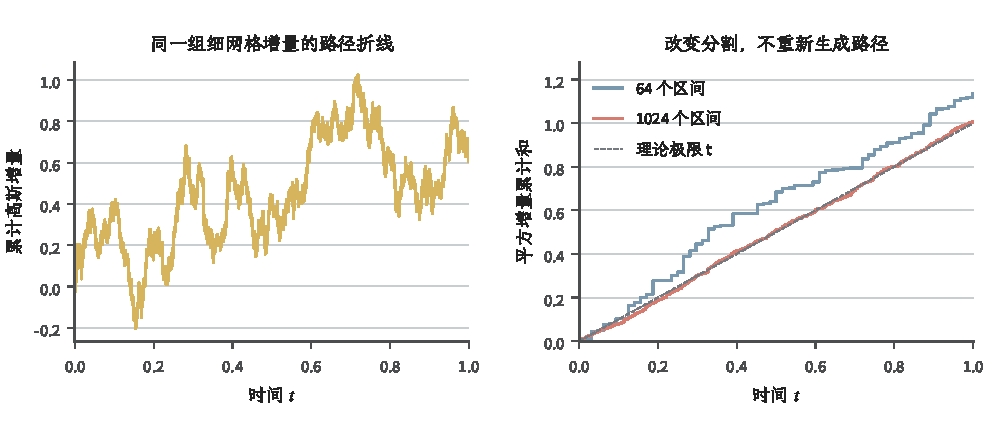
\includegraphics[width=\linewidth]{figures/math-preparation/reader-revision-dynamics/brownian-quadratic-variation.pdf}
  \caption{以固定随机种子构造的高斯增量教学例。左图由$4096$个独立增量
  $\Delta W_i\sim\mathcal N(0,1/4096)$累计成路径折线；右图将同一组增量分别合并为
  $64$和$1024$个时间区间，再累计各区间增量的平方。蓝、红阶梯线使用不同分割，
  灰色参考线为理论二次变差$t$。这里只绘制有限网格，不把某一条折线作为连续布朗路径或收敛证明。}
  \label{fig:reader-brownian-quadratic-variation}
\end{figure*}

平方增量会留下有限的累计量，这使普通积分的链式法则不再适用。接下来先构造只能使用过去信息的随机积分，再用它定义状态方程及其密度演化。

\subsection{可预测过程与Itô积分}

随机积分需要禁止被积量提前使用下一段噪声。可预测性把这项信息限制写成过程的可测条件；
在下面的简单过程中，它表现为每个区间的系数必须在该区间开始时已经知道。
一般可预测过程相对于由左连续适应过程生成的可预测$\sigma$代数可测；
这比逐时刻适应还包含时间方向的联合可测性。先对可预测简单过程定义积分。 给定分割$0=t_{0}<\cdots<t_{n}=T$， 令
\[
	H_{t}= \sum_{i=0}^{n-1}H_{i}\mathbb{I}_{(t_i,t_{i+1}]}(t),
\]
其中$H_{i}$对$\mathcal{F}_{t_i}$可测且平方可积。 定义
\begin{equation}
	\int_{0}^{T}H_{t}\,\mathrm{d}W_{t}:=
	\sum_{i=0}^{n-1}H_{i}(W_{t_{i+1}}-W_{t_i}). \label{eq:dynamical-simple-ito-integral}
\end{equation}
左端点可测性表示$H_{i}$可以依赖过去， 却不能利用尚未发生的布朗增量。

令
\[
	M_t=\int_0^t H_s\,\mathrm{d}W_s
	=\sum_{i=0}^{n-1}H_i
	\left(W_{t\wedge t_{i+1}}-W_{t\wedge t_i}\right).
\]
这个过程对$\mathcal F_t$适应且平方可积。对$0\leq s<t\leq T$，把
$M_t-M_s$按分割区间展开。对包含$s$的区间，系数已经对$\mathcal F_s$可测，
而$s$之后的增量独立于$\mathcal F_s$；对每个起点$t_i\geq s$的完整区间，塔式性质给出
\[
	\mathbb{E}[H_i\Delta W_i\mid\mathcal F_s]
	=
	\mathbb{E}\!\left[
	\mathbb{E}[H_i\Delta W_i\mid\mathcal F_{t_i}]
	\mid\mathcal F_s
	\right]
	=0.
\]
因此
\[
	\mathbb{E}[M_t-M_s\mid\mathcal F_s]=0,
	\qquad
	\mathbb{E}[M_t\mid\mathcal F_s]=M_s.
\]
所以$(M_t)_{0\leq t\leq T}$是平方可积鞅，特别地$\mathbb{E}[M_T]=0$。

等距关系还需要核对平方展开中的交叉项。记
$\Delta W_i=W_{t_{i+1}}-W_{t_i}$。当$i<j$时，
$H_iH_j\Delta W_i$对$\mathcal F_{t_j}$可测，故
\[
	\mathbb{E}[H_iH_j\Delta W_i\Delta W_j]
	=
	\mathbb{E}\!\left[
	H_iH_j\Delta W_i
	\mathbb{E}[\Delta W_j\mid\mathcal F_{t_j}]
	\right]
	=0.
\]
对角项则由$\Delta W_i$独立于$\mathcal F_{t_i}$及其方差
$t_{i+1}-t_i$得到
\[
	\mathbb{E}[H_i^2(\Delta W_i)^2]
	=\mathbb{E}[H_i^2](t_{i+1}-t_i).
\]
将各项相加，得到\term{Itô等距}（Itô isometry）
\begin{equation}
	\mathbb{E}\left[ \left( \int_{0}^{T}H_{t}\,\mathrm{d}W_{t}\right)^{2}\right] = \mathbb{E}
	\int_{0}^{T}H_{t}^{2}\,\mathrm{d}t. \label{eq:dynamical-ito-isometry}
\end{equation}
对可预测过程$H$，若满足 $\mathbb{E}\int_{0}^{T}H_{t}^{2}\,\mathrm{d}t<\infty$，
便可用可预测简单过程在该二阶范数下逼近，并借助等距关系把积分连续延拓。
条件期望是$L^2$压缩映射，因此上述鞅等式也在这个极限下保留：
$M_t=\int_0^tH_s\,\mathrm dW_s$仍是平方可积鞅。
也可以从渐进可测且满足同一平方可积条件的过程出发； 在通常滤过条件下，可取与它
在$\mathbb{P}\otimes\mathrm{d}t$意义下等价的可预测版本，因而得到相同的积分对象。
仅有适应性并不足以保证上述逼近与积分定义成立。

若使用右端点或中点， 被积量会含有当前增量的信息， 极限一般不同。
Stratonovich积分采用对称极限并保留普通链式法则，
Itô积分采用左端适应性并产生二次变差修正。 两种约定都合法，
但模型漂移在二者转换时会改变，不能只换积分符号
\scite{math-oksendal2003sde}

左端点约定还可以用一个有限和看清。记$\Delta W_i=W_{t_{i+1}}-W_{t_i}$，逐项
展开平方得
\[
  W_{t_{i+1}}^2-W_{t_i}^2
  =2W_{t_i}\Delta W_i+(\Delta W_i)^2.
\]
相加后，中间平方项望远镜消去；二次变差又使$\sum_i(\Delta W_i)^2\to T$，于是
$\sum_iW_{t_i}\Delta W_i\to(W_T^2-T)/2$。若改用右端点，相同恒等式给出
$(W_T^2+T)/2$。差别恰好是$T$，即被积量是否含有当前增量所留下的额外相关项。
这也预示下一节的Itô二阶修正，不能用“步长很小”把它删掉。

\subsection{随机微分方程与强解}

先明确多维驱动对象。相对于同一滤过，
$m$维标准布朗运动
$\bm W_t=(W_t^{(1)},\ldots,W_t^{(m)})^\top$
由相互独立的实值标准布朗运动组成。对$0\leq s<t$，增量
$\bm W_t-\bm W_s$独立于$\mathcal F_s$，并满足
\[
	\bm W_t-\bm W_s\sim\mathcal N(\bm0,(t-s)\bm I_m),
	\qquad
	[W^{(i)},W^{(j)}]_t=\delta_{i,j}t.
\]
最后一个等式说明不同分量的交叉二次变差为零，而每个分量的二次变差为$t$。

布朗路径没有普通时间导数，因此下式的微分记号只是一种紧凑写法，真正定义来自积分等式。
\begin{definition}[Itô随机微分方程与强解]
\label{def:dynamical-ito-sde-strong-solution}
$d$维状态由这个$m$维布朗运动驱动时，Itô\term{随机微分方程}（stochastic differential equation, SDE）写成
\begin{equation}
	\mathrm{d}\bm{X}_{t}= \bm{b}(t,\bm{X}_{t})\,\mathrm{d}t + \bm{\sigma}(t,\bm{X}_{t}
	)\,\mathrm{d}\bm{W}_{t}. \label{eq:dynamical-ito-sde}
\end{equation}
其中$\bm{b}:[0,T]\times\mathbb{R}^d\to\mathbb{R}^d$是漂移，
$\bm{\sigma}:[0,T]\times\mathbb{R}^d\to\mathbb{R}^{d\times m}$是扩散系数，二者均联合Borel可测。
它的含义是
\[
	\bm{X}_{t}= \bm{X}_{0}+ \int_{0}^{t}\bm{b}(s,\bm{X}_{s})\,\mathrm{d}s+ \int_{0}
	^{t}\bm{\sigma}(s,\bm{X}_{s})\,\mathrm{d}\bm{W}_{s}.
\]
在给定的滤过概率空间上，$\bm W$是相对于该滤过的布朗运动，初值$\bm X_0$对
$\mathcal F_0$可测。若一个连续过程对由$\bm X_0$与$(\bm W_s)_{0\leq s\leq t}$生成、
完成并取右连续版本的滤过适应，使两个积分都有定义，
并且上式以概率$1$对所有$t\in[0,T]$同时成立，就称它为该方程的\term{强解}
（strong solution）。
\end{definition}
这里的“强”强调解由给定初值与布朗运动的过去生成，无需另添随机信息，而不只指定
解的分布。路径唯一性是指同一空间上使用同一初值和布朗运动的两个适应连续解
几乎必然处处相同。

\begin{theorem}[SDE强解的存在唯一性]
	\label{thm:dynamical-sde-strong-existence}
	设$(\mathcal F_t)_{t\geq0}$满足通常条件，即完备且右连续，
	$\bm W$是相对于该滤过的$m$维标准布朗运动，
	$\bm{X}_0$对$\mathcal{F}_0$可测且
	$\mathbb{E}\lVert\bm{X}_0\rVert_2^2<\infty$。
	设$\bm b$与$\bm\sigma$关于$(t,\bm x)$联合Borel可测。
	若存在常数$L,C$，使对所有$t\in[0,T]$及$\bm{x},\bm{y}\in\mathbb{R}^d$，
	\begin{align*}
		\lVert\bm{b}(t,\bm{x})-\bm{b}(t,\bm{y})\rVert_2
		+\lVert\bm{\sigma}(t,\bm{x})-\bm{\sigma}(t,\bm{y})\rVert_{\mathrm{F}}
		&\leq L\lVert\bm{x}-\bm{y}\rVert_2,\\
		\lVert\bm{b}(t,\bm{x})\rVert_2^2
		+\lVert\bm{\sigma}(t,\bm{x})\rVert_{\mathrm{F}}^2
		&\leq C(1+\lVert\bm{x}\rVert_2^2),
	\end{align*}
	则式~\eqref{eq:dynamical-ito-sde}在$[0,T]$上存在唯一强解，并且
	$\mathbb{E}\sup_{t\leq T}\lVert\bm{X}_t\rVert_2^2<\infty$。
\end{theorem}

证明仍采用Picard迭代，但确定性积分的上界要与Itô等距和鞅最大不等式配合。
在足够短的时间区间上，这些估计使迭代成为二阶过程空间中的压缩；
逐段延拓覆盖$[0,T]$。对两组解作差并使用同样估计，再由Grönwall不等式得到路径唯一性。
线性增长界控制二阶矩并排除有限时间爆炸。若只有局部Lipschitz，以上论证先给出爆炸时刻之前的局部唯一解，
还需额外增长或Lyapunov条件证明爆炸时刻几乎必然大于$T$。

\subsection{Itô公式与二次变差修正}

\begin{theorem}[Itô公式]
	\label{thm:dynamical-ito-formula} 设$\bm{X}_{t}$满足 式~\eqref{eq:dynamical-ito-sde}，
	并令$f(t,\bm{x})$关于$t$一阶连续可微、 关于$\bm{x}$二阶连续可微。 在相应可积条件下，
	\begin{align}
		\mathrm{d}f(t,\bm{X}_{t}) & = \left[ \partial_{t}f + \nabla f^{\top}\bm{b}+ \frac{1}{2}\operatorname{tr}\left( \bm{\sigma}\bm{\sigma}^{\top}\nabla^{2}f \right) \right]\mathrm{d}t \notag \\
		                          & \quad+ \nabla f^{\top}\bm{\sigma}\,\mathrm{d}\bm{W}_{t}, \label{eq:dynamical-ito-formula}
	\end{align}
	其中右侧各函数在$(t,\bm{X}_{t})$处取值。
\end{theorem}

\paragraph{证明路线与关键项。}
先在分割上对 $f(t_{i+1},\bm{X}_{t_{i+1}}) -f(t_{i},\bm{X}_{t_i})$ 作二阶Taylor展开。
状态增量为
\[
	\Delta\bm{X}_{i}
	=\bm{b}_{i}\Delta t_{i}+\bm{\sigma}_{i}\Delta\bm{W}_{i}+\text{高阶余项}.
\]
一阶项产生 $\partial_{t}f\,\Delta t_{i}$、
$\nabla f^{\top}\bm{b}_{i}\Delta t_{i}$ 和
$\nabla f^{\top}\bm{\sigma}_{i}\Delta\bm{W}_{i}$。 二阶项中， $(\Delta t_{i})^{2}$及
$\Delta t_{i}\Delta W_{i}$求和后消失； 而 $\Delta\bm{W}_{i}\Delta\bm{W}_{i}^{\top}$
的和依二次变差趋向$\bm{I}\Delta t_{i}$。 因此留下
\[
		\frac{1}{2}\operatorname{tr}
		(\bm{\sigma}\bm{\sigma}^{\top}\nabla^{2}f)\Delta t_{i}.
\]
完整证明还需先用停时把$\bm{X}$、系数及$f$的导数局部化到有界区域，再以简单可预测过程逼近随机被积项，
并分别证明Taylor余项、漂移和二次变差交叉项在相应概率或$L^{1}$意义下收敛； 最后令停时趋向无穷。
这里给出的展开只说明二阶修正项的来源，不替代这些局部化、逼近与收敛论证。

形式记忆规则
\[
	(\mathrm{d}W_{t})^{2}=\mathrm{d}t, \qquad \mathrm{d}W_{t}\,\mathrm{d}t=0, \qquad
	(\mathrm{d}t)^{2}=0
\]
概括了量级， 但不能替代适应性、可积性与极限证明。

两个基本例子可以核对积分约定。常数被积过程给出
$\int_0^T c\,\mathrm{d}W_t=cW_T$。对$f(x)=x^2$应用Itô公式则有
\[
	W_T^2=2\int_0^T W_t\,\mathrm{d}W_t+T,
	\qquad
	\int_0^T W_t\,\mathrm{d}W_t=\frac{W_T^2-T}{2}.
\]
若误用普通链式法则，就会漏掉由二次变差产生的$-T/2$修正。

\subsection{线性SDE与Ornstein--Uhlenbeck过程}

先考虑确定性系数的向量线性SDE
\[
	\mathrm d\bm X_t
	=(\bm A_t\bm X_t+\bm c_t)\,\mathrm dt
	+\bm G_t\,\mathrm d\bm W_t,
\]
其中$\bm A_t\in\mathbb{R}^{d\times d}$和$\bm c_t\in\mathbb{R}^d$
是确定性的局部可积函数，$\bm G_t\in\mathbb{R}^{d\times m}$是确定性函数且
$\lVert\bm G_t\rVert_{\mathrm F}^2$局部可积，并假设
$\bm X_0\in L^2$。这些条件保证方程有唯一平方可积强解；相应的均值与协方差函数
绝对连续，下面的微分方程对几乎处处的$t$成立。记
\[
	\bm m_t=\mathbb{E}[\bm X_t],\qquad
	\bm P_t=\operatorname{Cov}(\bm X_t).
\]
对积分方程取期望，随机积分的鞅性质给出
\begin{equation}
	\dot{\bm m}_t=\bm A_t\bm m_t+\bm c_t.
	\label{eq:dynamical-linear-sde-mean}
\end{equation}
再令$\widetilde{\bm X}_t=\bm X_t-\bm m_t$，则
$\mathrm d\widetilde{\bm X}_t
=\bm A_t\widetilde{\bm X}_t\,\mathrm dt+\bm G_t\,\mathrm d\bm W_t$。
对矩阵乘积使用Itô公式，
\[
	\begin{aligned}
	\mathrm d(\widetilde{\bm X}_t\widetilde{\bm X}_t^\top)
	={}&
	\left(
	\bm A_t\widetilde{\bm X}_t\widetilde{\bm X}_t^\top
	+\widetilde{\bm X}_t\widetilde{\bm X}_t^\top\bm A_t^\top
	+\bm G_t\bm G_t^\top
	\right)\mathrm dt\\
	&+\bm G_t\,\mathrm d\bm W_t\,\widetilde{\bm X}_t^\top
	+\widetilde{\bm X}_t\,\mathrm d\bm W_t^\top\bm G_t^\top.
	\end{aligned}
\]
取期望后两个随机积分项消失，得到
\begin{equation}
	\dot{\bm P}_t
	=\bm A_t\bm P_t+\bm P_t\bm A_t^\top+\bm G_t\bm G_t^\top.
	\label{eq:dynamical-linear-sde-covariance}
\end{equation}
这两式说明，漂移传播已有均值与协方差，扩散项则持续注入协方差；
它们是离散Kalman预测公式在连续时间中的对应关系。

标量Ornstein--Uhlenbeck过程是上述方程取
$\bm A_t=-\lambda$、$\bm c_t=0$和$\bm G_t=\sigma$的特例：
\begin{equation}
	\mathrm{d}X_{t}= -\lambda X_{t}\,\mathrm{d}t+ \sigma\,\mathrm{d}W_{t}, \qquad \lambda
	>0. \label{eq:dynamical-ou-sde}
\end{equation}
对$\mathrm{e}^{\lambda t}X_{t}$使用Itô公式， 交叉二次变差项因确定性因子有限变差而为零，
得到
\[
	X_{t}= \mathrm{e}^{-\lambda t}X_{0}+ \sigma \int_{0}^{t}\mathrm{e}^{-\lambda(t-s)}
	\,\mathrm{d}W_{s}.
\]
若$X_{0}$与布朗运动独立，
\begin{align}
	\mathbb{E}X_{t}           & = \mathrm{e}^{-\lambda t}\mathbb{E}X_{0}, \label{eq:dynamical-ou-mean}                                                                          \\
	\operatorname{Var}(X_{t}) & = \mathrm{e}^{-2\lambda t}\operatorname{Var}(X_{0}) + \frac{\sigma^{2}}{2\lambda}(1-\mathrm{e}^{-2\lambda t}). \label{eq:dynamical-ou-variance}
\end{align}
第二式由Itô等距得到。 均值衰减到零， 方差却趋向$\sigma^{2}/(2\lambda)$。 随机稳定状态不是所有轨迹收敛到零，
而是阻尼与持续噪声形成平稳分布。当$\sigma\neq0$时，该分布为非退化的
$\mathcal N(0,\sigma^2/(2\lambda))$；当$\sigma=0$时，它退化为$\delta_0$。

也可对$f(x)=x^{2}$用Itô公式：
\[
	\mathrm{d}(X_{t}^{2}) = (-2\lambda X_{t}^{2}+\sigma^{2})\,\mathrm{d}t + 2\sigma
	X_{t}\,\mathrm{d}W_{t}.
\]
取期望后随机积分均值为零， 得到二阶矩ODE， 其解与式~\eqref{eq:dynamical-ou-variance}一致。
若漏掉Itô修正$\sigma^{2}\mathrm{d}t$， 便会错误地预测方差也衰减到零。

\subsection{生成元与Fokker--Planck方程}

路径方程已经说明一个状态如何移动；若只关心分布，则需计算任意光滑读数$\varphi(\bm X_t)$
的平均变化率。生成元把这项短时变化浓缩成作用于$\varphi$的微分算子。
设$\bm a=\bm\sigma\bm\sigma^\top$。对光滑紧支撑测试函数$\varphi$，时刻$t$的生成元为
\begin{definition}[Itô扩散的生成元]
\label{def:dynamical-diffusion-generator}
\[
	(\mathcal{L}_t\varphi)(\bm{x})
	=\bm{b}(t,\bm{x})^{\top}\nabla\varphi(\bm{x})
	+\frac12\operatorname{tr}\!\left(\bm{a}(t,\bm{x})\nabla^2\varphi(\bm{x})\right).
\]
\end{definition}
在系数连续且短时期望允许相应极限交换时，它也等于从$\bm x$出发的
$[\mathbb E_{t,\bm x}\varphi(\bm X_{t+h})-\varphi(\bm x)]/h$在$h\downarrow0$时的极限。
生成元作用于读数函数；Fokker--Planck算子稍后作用于密度，二者通过积分对偶相连。
在Itô公式中的随机积分可积且均值为零时，取期望得到弱演化式
\[
	\frac{\mathrm{d}}{\mathrm{d}t}\mathbb{E}[\varphi(\bm{X}_{t})]
	=\mathbb{E}[(\mathcal{L}_t\varphi)(\bm{X}_t)].
\]
这个等式只描述分布对测试函数的作用，不预设$\bm{X}_t$具有处处光滑的密度。

若$\bm{X}_t$进一步具有密度$p(t,\bm{x})$，且系数与密度足够正则，
便可把弱式写成密度积分并对空间变量分部积分。边界项在测试函数紧支撑，
或密度与通量适当衰减的条件下消失，得到
\begin{equation}
	\partial_{t}p(t,\bm{x}) = - \sum_{i}\partial_{x_i}\bigl(b_{i}(t,\bm{x})p(t,\bm{x}
	)\bigr) + \frac{1}{2}\sum_{i,j}\partial_{x_i}\partial_{x_j}\bigl(a_{i,j}(t, \bm
	{x})p(t,\bm{x})\bigr). \label{eq:dynamical-fokker-planck}
\end{equation}
这就是\term{Fokker--Planck方程}。 它是SDE生成元的伴随方程， 描述各时刻边缘密度怎样流动和扩散。

推导先在弱意义下成立。 要把它解释为逐点经典偏微分方程，
还需密度存在、系数正则性与边界条件。 退化扩散矩阵可能使密度集中在低维集合，
此时相对于全维Lebesgue测度的光滑密度未必存在。

\subsection{SDE数值近似、Langevin与概率流}

Euler--Maruyama方法把 式~\eqref{eq:dynamical-ito-sde}离散为
\begin{equation}
	\bm{X}_{k+1}= \bm{X}_{k}+ \bm{b}(t_{k},\bm{X}_{k})h+ \bm{\sigma}(t_{k},\bm{X}_{k}
	)\sqrt{h}\,\bm{\varepsilon}_{k}, \qquad \bm{\varepsilon}_{k}\sim\mathcal{N}(\bm
	{0},\bm{I}). \label{eq:dynamical-euler-maruyama}
\end{equation}
式中的独立$\bm\varepsilon_k$为$m$维标准高斯。讨论强误差时，必须令
$\sqrt h\,\bm\varepsilon_k=\bm W_{t_{k+1}}-\bm W_{t_k}$，使数值解与真解使用同一个驱动。
对自治系数，若$\bm{b}$与$\bm{\sigma}$全局Lipschitz并满足线性增长条件，且初值平方可积，
则在固定有限时域的网格点上有代表性的强误差界
\[
	\max_{0\leq k\leq T/h}
	\left(\mathbb{E}\lVert\bm{X}_{t_k}-\bm{X}_k\rVert_2^2\right)^{1/2}
	\leq C_T h^{1/2}.
\]
若系数还显式依赖时间，需要相应的时间正则性。一个便于陈述的弱一阶充分条件是：
自治的漂移、扩散系数和测试函数$\varphi$具有至四阶连续有界导数，并满足所需矩条件。此时
\[
	\left|\mathbb{E}\varphi(\bm{X}_T)-\mathbb{E}\varphi(\bm{X}_{T/h})\right|
	\leq C_{\varphi,T}h.
\]
强误差比较同一布朗路径上的数值解与真解，弱误差比较测试函数期望；
两者的对象不同，弱阶更高不表示逐路径更准确。加性噪声或更强结构可以提高特定方法的阶，
但不能把这些特殊结论当作一般乘性噪声的保证。

过阻尼Langevin SDE
\begin{equation}
	\mathrm{d}\bm{X}_{t}= \frac{1}{2}\nabla\log\pi(\bm{X}_{t})\,\mathrm{d}t+ \mathrm{d}
	\bm{W}_{t}\label{eq:dynamical-langevin-sde}
\end{equation}
在$\pi$光滑、可归一化且边界通量消失等条件下， 把$p=\pi$代入Fokker--Planck方程可见漂移通量与扩散通量相消，
所以$\pi$是不变密度。 这只证明保持性。 从任意初值收敛到$\pi$还需要遍历性与约束势能等条件，
离散后的未校正Langevin算法还会产生步长偏差。

扩散生成模型设计随时间加噪的前向SDE， 再学习与边缘分数$\nabla\log p_{t}$有关的反向动态。
与同一边缘密度族对应的概率流ODE可以写成
\[
	\frac{\mathrm{d}\bm{X}_{t}}{\mathrm{d}t}= \bm{b}(t,\bm{X}_{t}) - \frac{1}{2}\bm
	{a}(t) \nabla\log p_{t}(\bm{X}_{t})
\]
这一简式要求扩散矩阵只依赖时间； 状态依赖扩散还会出现额外散度项。
概率流ODE匹配边缘密度演化， 不表示它与SDE具有相同样本路径。
反向生成还需要分数估计与时间反演条件， 不能只凭前向Fokker--Planck方程自动得到。

从单条轨迹转向密度时，控制的对象也改变了。表~\ref{tab:dynamical-path-distribution}
将本节的几种结论放在一起：保持一个分布与从任意初态趋向该分布之间，还隔着长期
混合条件；具有相同边缘密度则连联合路径分布也没有固定。

\begin{table*}[htbp]
  \centering
  \begin{tabularx}{\linewidth}{lXX}
    \toprule
    结论 & 所比较的对象 & 仍需另外说明的对象\\
    \midrule
    强数值误差小 & 同一噪声路径下的数值状态与真状态 & 目标分布的长期抽样偏差\\
    弱数值误差小 & 测试函数在两种状态分布下的期望 & 单条路径之间的距离\\
    密度$\pi$不变 & 若初始分布为$\pi$，以后仍为$\pi$ & 其他初态是否收敛到$\pi$\\
    概率流匹配边缘 & 每个时刻的状态分布 & 时间间联合分布与样本路径\\
    \bottomrule
  \end{tabularx}
  \caption{随机演化中不同结论的对象。强弱误差须满足相应数值方法条件；不变性和边缘
  匹配须满足前述正则性及边界条件。表中各项不能互相替代。}
  \label{tab:dynamical-path-distribution}
\end{table*}

\section{保持保守轨迹的几何结构并构造采样提议}
\label{sec:dynamical-hamiltonian-geometric-integration}

前面的随机微分研究噪声与分布演化。本节回到确定性状态方程，
专门研究具有位置--动量结构的系统：能量守恒和相空间体积保持成为应保留的性质。
几何积分据此设计数值更新；Hamilton蒙特卡洛再加入随机刷新与接受校正，
才能把这种确定性轨迹用于概率采样。它不是由一般SDE直接推出的一项性质。

\subsection{相空间状态与Hamilton方程}

前面主要问扰动是否衰减。 保守系统关心另一类结构：
动态可以长期移动，却保持总能量和相空间体积。
\begin{definition}[可分Hamilton系统]
\label{def:dynamical-separable-hamiltonian-system}
令位置$\bm{q}\in\mathbb{R}^{d}$、动量$\bm{p}\in\mathbb{R}^{d}$，设势能$U$连续可微，
质量矩阵$\bm M\in\mathbb R^{d\times d}$对称正定。可分Hamilton量为
\begin{equation}
	H(\bm{q},\bm{p}) = U(\bm{q})+ \frac{1}{2}\bm{p}^{\top}\bm{M}^{-1}\bm{p}, \qquad
	\bm{M}\succ\bm{0}. \label{eq:dynamical-separable-hamiltonian}
\end{equation}
Hamilton方程为
\begin{equation}
	\dot{\bm{q}}= \nabla_{\bm{p}}H, \qquad \dot{\bm{p}}= -\nabla_{\bm{q}}H. \label{eq:dynamical-hamilton-equations}
\end{equation}
\end{definition}
第一式把动量变成位置速度， 第二式让势能梯度改变动量。 这不是沿$-\nabla H$下降，
而是用辛矩阵
\[
	\bm{J}=
	\begin{bmatrix}
		\bm{0}  & \bm{I} \\
		-\bm{I} & \bm{0}
	\end{bmatrix}
\]
旋转Hamilton梯度。

\subsection{Hamilton流的能量守恒}

\begin{theorem}[Hamilton能量守恒]
	\label{thm:dynamical-hamiltonian-energy-conservation} 若$H$连续可微、不显含时间，
	且Hamilton方程的解在所考察区间存在， 则沿精确轨迹
	\[
		H(\bm{q}(t),\bm{p}(t)) = H(\bm{q}(0),\bm{p}(0)).
	\]
\end{theorem}

\begin{proof}
	沿轨迹使用链式法则，
	\[
		\begin{aligned}
			\frac{\mathrm{d}}{\mathrm{d}t}H & = \nabla_{\bm{q}}H^{\top}\dot{\bm{q}}+ \nabla_{\bm{p}}H^{\top}\dot{\bm{p}}              \\
			                                & = \nabla_{\bm{q}}H^{\top}\nabla_{\bm{p}}H - \nabla_{\bm{p}}H^{\top}\nabla_{\bm{q}}H =0.
		\end{aligned}
	\]
	因此Hamilton量沿每条存在的轨迹保持常数。
\end{proof}

若$H$显式依赖时间， 同一计算只给出
$\mathrm{d}H/\mathrm{d}t=\partial H/\partial t$。 若解在有限时间爆炸， 守恒结论也只适用于流存在的区间。
能量守恒不表示位置有界； 若势能的等能面不紧，轨迹仍可能逃向无穷远。

\subsection{相空间体积与辛结构}

把$\bm{z}=(\bm{q},\bm{p})$， 向量场写成 $\bm{F}(\bm{z})=\bm{J}\nabla H(\bm{z})$。
若$H$二阶连续可微，
\[
	\nabla\cdot\bm{F}= \operatorname{tr}(\bm{J}\nabla^{2}H)=0,
\]
因为$\bm{J}$反对称而$\nabla^{2}H$对称， 二者乘积的迹为零。

设流映射为$\varphi_{t}$， 其Jacobian矩阵为 $\bm{G}_{t}=\nabla\varphi_{t}(\bm{z}_{0})$。
变分方程给出
\[
	\dot{\bm{G}}_{t}= \nabla\bm{F}(\bm{z}(t))\bm{G}_{t}.
\]
Jacobi行列式公式于是给出
\[
	\frac{\mathrm{d}}{\mathrm{d}t}\log|\det\bm{G}_{t}| = \operatorname{tr}(\nabla\bm
	{F}) = \nabla\cdot\bm{F}=0.
\]
由于$\bm{G}_{0}=\bm{I}$， 有$|\det\bm{G}_{t}|=1$。
因此精确Hamilton流保持相空间体积。

体积只记录所有方向伸缩率的乘积，Hamilton系统还保持方向对之间的几何关系。
\begin{definition}[标准辛形式与辛映射]
\label{def:dynamical-symplectic-form-map}
对切向量$\bm{u},\bm{v}\in\mathbb{R}^{2d}$，定义\term{辛形式}（symplectic form）
\[
	\omega(\bm{u},\bm{v})=\bm{u}^{\top}\bm{J}\bm{v}.
\]
可微映射$\psi$称为辛映射，如果其Jacobian矩阵$\bm{G}=\nabla\psi$满足
\begin{equation}
	\bm{G}^{\top}\bm{J}\bm{G}=\bm{J}. \label{eq:dynamical-symplectic-map}
\end{equation}
其中等式在映射定义域的每一点成立，$\psi$为该域到$\mathbb R^{2d}$的连续可微映射。
\end{definition}
该等式表示映射前后的任意两方向具有相同辛形式值。

若$H\in C^2$，沿精确流有
$\nabla\bm{F}=\bm{J}\nabla^2H$。记$\bm{S}=\nabla^2H=\bm{S}^{\top}$，则
\[
	\begin{aligned}
	\frac{\mathrm{d}}{\mathrm{d}t}
	(\bm{G}_t^{\top}\bm{J}\bm{G}_t)
	&=\bm{G}_t^{\top}
	\left[(\bm{J}\bm{S})^{\top}\bm{J}
	+\bm{J}(\bm{J}\bm{S})\right]\bm{G}_t\\
	&=\bm{G}_t^{\top}(\bm{S}-\bm{S})\bm{G}_t=\bm{0}.
	\end{aligned}
\]
初值为$\bm{G}_0^{\top}\bm{J}\bm{G}_0=\bm{J}$，所以精确流满足
式~\eqref{eq:dynamical-symplectic-map}。对该式取行列式可得
$(\det\bm{G}_t)^2=1$；由$\det\bm{G}_0=1$和连续性知$\det\bm{G}_t=1$。
因此辛性蕴含定向体积保持。在一个位置与一个动量组成的二维相空间中，辛形式就是
有向面积形式；但当$d\geq2$时，一般的体积保持映射未必保持辛形式。例如在
$(q_1,q_2,p_1,p_2)$坐标下，$\operatorname{diag}(2,1,1,1/2)$的行列式为$1$，
却把第一对位置动量的面积乘以$2$、第二对乘以$1/2$，不满足
式~\eqref{eq:dynamical-symplectic-map}。总体积不变不能替代每对共轭方向的结构保持。

\subsection{分裂积分与蛙跳方法}

对可分Hamilton量~\eqref{eq:dynamical-separable-hamiltonian}， 一步步长为$h$的蛙跳积分写成
\begin{align}
	\bm{p}_{k+1/2} & = \bm{p}_{k}- \frac{h}{2}\nabla U(\bm{q}_{k}), \label{eq:dynamical-leapfrog-half-momentum}        \\
	\bm{q}_{k+1}   & = \bm{q}_{k}+ h\bm{M}^{-1}\bm{p}_{k+1/2}, \label{eq:dynamical-leapfrog-position}                  \\
	\bm{p}_{k+1}   & = \bm{p}_{k+1/2}- \frac{h}{2}\nabla U(\bm{q}_{k+1}). \label{eq:dynamical-leapfrog-final-momentum}
\end{align}
两次动量剪切和一次位置剪切都具有Jacobian矩阵的行列式$1$， 所以复合映射体积保持。 把$h$换成$-
h$并反向执行三步， 可以精确恢复起点， 所以映射具有时间可逆性。 它还是辛积分器， 因为每个子步都是一个Hamilton子流。

这些性质可以直接从Jacobian核对。动量剪切
$S_U^c(\bm{q},\bm{p})=(\bm{q},\bm{p}-c\nabla U(\bm{q}))$与位置剪切
$S_K^h(\bm{q},\bm{p})=(\bm{q}+h\bm{M}^{-1}\bm{p},\bm{p})$的Jacobian分别为
\[
	\bm{G}_U=
	\begin{bmatrix}
		\bm{I}&\bm{0}\\
		-c\nabla^2U&\bm{I}
	\end{bmatrix},
	\qquad
	\bm{G}_K=
	\begin{bmatrix}
		\bm{I}&h\bm{M}^{-1}\\
		\bm{0}&\bm{I}
	\end{bmatrix}.
\]
由于$\nabla^2U$与$\bm{M}^{-1}$对称，直接相乘可得
$\bm{G}_U^{\top}\bm{J}\bm{G}_U=\bm{J}$和
$\bm{G}_K^{\top}\bm{J}\bm{G}_K=\bm{J}$。
蛙跳映射是$S_U^{h/2}\circ S_K^h\circ S_U^{h/2}$，而辛映射的复合仍为辛映射。
每个三角Jacobian的行列式为$1$，也再次给出体积保持。

令动量翻转为$R(\bm{q},\bm{p})=(\bm{q},-\bm{p})$，并记一步蛙跳为$\Psi_h$。
三步的对称排列给出
\[
	R\circ\Psi_h\circ R=\Psi_h^{-1}=\Psi_{-h}.
\]
所以可逆性不是简单的$\Psi_h=\Psi_h^{-1}$，而是在反向运动时同时翻转动量。

蛙跳法一般不精确保持原Hamilton量。 它对固定有限时间具有二阶全局精度，
并在合适光滑和步长条件下近似保持一个修正Hamilton量，
所以长时间能量误差常表现为有界振荡，而非单向漂移。
“可逆”“体积保持”“辛”和“能量误差小”是相关但不同的性质；
验证其中一项不能自动推出其余各项。

\begin{example}[谐振子的精确与数值轨道]
	\label{ex:dynamical-harmonic-oscillator} 取$U(q)=q^{2}/2$、$M=1$。 Hamilton方程为
	\[
		\dot q=p,\qquad \dot p=-q,
	\]
	精确轨迹沿圆 $q^{2}+p^{2}=\text{常数}$旋转。蛙跳一步可写成
	\[
		\begin{bmatrix}q_{k+1}\\p_{k+1}\end{bmatrix}
		=
		\begin{bmatrix}
			1-h^2/2 & h\\
			-h+h^3/4 & 1-h^2/2
		\end{bmatrix}
		\begin{bmatrix}q_k\\p_k\end{bmatrix}.
	\]
	该矩阵行列式为$1$、迹为$2-h^2$。其特征值在单位圆上且不退化的条件是
	$|2-h^2|<2$，即$0<h<2$。在这个稳定范围内，数值轨迹沿接近圆的闭曲线运动，
	原能量会有小幅周期误差； 步长过大时，即使每一步仍可逆且行列式为$1$，
	轨迹也可能不稳定。 几何结构保持不能替代步长稳定性检查。
\end{example}

\subsection{Hamilton蒙特卡洛与接受校正}

若目标密度满足 $\pi(\bm{q})\propto\exp[-U(\bm{q})]$， 再引入高斯动量
$\bm{p}\sim \mathcal{N}(\bm{0},\bm{M})$， 联合密度正比于 $\exp[-H(\bm{q},\bm{p})]$。
精确Hamilton流同时保持$H$和体积， 因而保持该联合密度。 数值蛙跳产生候选
$(\bm{q}',\bm{p}')$时存在能量误差
\[
	\Delta H = H(\bm{q}',\bm{p}')-H(\bm{q},\bm{p}).
\]
Metropolis接受概率
\begin{equation}
	a = \min\{1,\exp(-\Delta H)\} \label{eq:dynamical-hmc-acceptance}
\end{equation}
结合可逆、体积保持的提议映射， 恢复对目标联合分布的详细平衡。 拒绝时保留原位置， 动量翻转用于明确反向提议。

更具体地，令$\rho(\bm{z})\propto\exp[-H(\bm{z})]$，把若干步蛙跳与末端动量翻转合成映射
$T$。上面的可逆性给出$T(T(\bm{z}))=\bm{z}$，体积保持给出
$|\det\nabla T|=1$。于是成对状态间的接受概率满足
\[
	\rho(\bm{z})\min\!\left\{1,\frac{\rho(T\bm{z})}{\rho(\bm{z})}\right\}
	=\min\{\rho(\bm{z}),\rho(T\bm{z})\}
	=\rho(T\bm{z})\min\!\left\{1,\frac{\rho(\bm{z})}{\rho(T\bm{z})}\right\}.
\]
这就是确定性提议上的详细平衡；Jacobian若不为$1$，接受比还必须包含相应体积因子。
每轮重新抽取服从$\mathcal{N}(\bm{0},\bm{M})$的动量也保持联合目标密度，
边缘化动量后才得到位置目标$\pi(\bm{q})$。

接受校正保证的是不变分布， 不是独立样本、快速混合或有限预算精度。
步长太大会导致频繁拒绝， 轨迹太短会导致高自相关，
质量矩阵不合适会使不同方向的时间尺度失配。
另一方面，Hamilton轨迹不要求能量持续下降。
采样希望沿等能面远距离移动后保持目标分布， 优化则希望找到低目标值；
把Hamilton动力学解释成“更快的梯度下降”会混淆这两个目标。

\section{本章小结}
\label{sec:dynamical-systems-state-estimation-summary}

状态把过去对未来的作用压缩进当前变量。 给定初值与输入，差分方程直接生成递推，
常微分方程通过流映射生成连续轨迹。 局部Lipschitz条件保证局部唯一解，
全局解还需要增长或有界性控制。 线性时不变系统可用矩阵指数求解，
时变系统则需要保留状态转移矩阵的时间顺序。

离散化近似连续流。 Euler、Runge--Kutta与零阶保持的误差来源不同，
连续系统稳定也不保证任意步长的数值递推稳定。 仿射更新的结合律允许前缀扫描，
却不允许交换时间次序。 稳定性同样要区分平衡点不离开、轨迹趋近平衡和输入作用。
谱决定线性系统的长期行为， Lyapunov函数把更一般的稳定性转成标量下降，
非正规系统则提醒我们长期衰减可以伴随短时放大。

加入过程噪声后，状态方程传播分布； 加入观测噪声后，观测历史通过条件化形成滤波分布。
在线性高斯及独立噪声条件下， Kalman递推由一次联合高斯条件化精确得到， RTS递推再利用未来观测修正过去边缘。
这些是有限时域结论。 稳态增益和极限协方差还需要第~\ref{chap:control-theory}章建立的可检测性等系统条件，
非线性或非高斯模型也需要明确近似对象。

随机参数递推的平均ODE只描述平均方向。
非对称线性漂移应检查特征值实部、对称部分或Lyapunov方程，
不能把一般漂移矩阵当作目标Hessian矩阵。 同策略线性TD的加权Markov收缩可给出稳定漂移，
离策略分布改变后必须重新证明。 平均稳定仍不能替代步长、噪声、混合和迭代有界性。

连续时间噪声具有平方根增量和非零二次变差。 这使布朗路径不能作为普通可微输入， 并使Itô公式保留二阶修正。
SDE描述随机路径， Fokker--Planck方程描述边缘密度， Euler--Maruyama的强弱误差又是数值近似性质。
Hamilton动力学则保持能量与相空间几何； 蛙跳的可逆和体积保持帮助构造采样提议， 但不等于精确守恒，也不等于优化下降。

由此，章首问题可以分成两部分回答： 状态方程和噪声条件决定轨迹或分布怎样演化，
观测历史和条件化规则决定能够推断什么。 第~\ref{chap:decision-theory-and-dynamic-risk}章将在这些动态之上评价行动后果，
第~\ref{chap:control-theory}章再让输入由反馈主动选择，
并建立稳态估计、最优控制与安全约束所需的结构条件。
